% Options for packages loaded elsewhere
\PassOptionsToPackage{unicode}{hyperref}
\PassOptionsToPackage{hyphens}{url}
\PassOptionsToPackage{dvipsnames,svgnames,x11names}{xcolor}
%
\documentclass[
  letterpaper,
  DIV=11,
  numbers=noendperiod]{scrreprt}

\usepackage{amsmath,amssymb}
\usepackage{iftex}
\ifPDFTeX
  \usepackage[T1]{fontenc}
  \usepackage[utf8]{inputenc}
  \usepackage{textcomp} % provide euro and other symbols
\else % if luatex or xetex
  \usepackage{unicode-math}
  \defaultfontfeatures{Scale=MatchLowercase}
  \defaultfontfeatures[\rmfamily]{Ligatures=TeX,Scale=1}
\fi
\usepackage{lmodern}
\ifPDFTeX\else  
    % xetex/luatex font selection
\fi
% Use upquote if available, for straight quotes in verbatim environments
\IfFileExists{upquote.sty}{\usepackage{upquote}}{}
\IfFileExists{microtype.sty}{% use microtype if available
  \usepackage[]{microtype}
  \UseMicrotypeSet[protrusion]{basicmath} % disable protrusion for tt fonts
}{}
\makeatletter
\@ifundefined{KOMAClassName}{% if non-KOMA class
  \IfFileExists{parskip.sty}{%
    \usepackage{parskip}
  }{% else
    \setlength{\parindent}{0pt}
    \setlength{\parskip}{6pt plus 2pt minus 1pt}}
}{% if KOMA class
  \KOMAoptions{parskip=half}}
\makeatother
\usepackage{xcolor}
\setlength{\emergencystretch}{3em} % prevent overfull lines
\setcounter{secnumdepth}{3}
% Make \paragraph and \subparagraph free-standing
\makeatletter
\ifx\paragraph\undefined\else
  \let\oldparagraph\paragraph
  \renewcommand{\paragraph}{
    \@ifstar
      \xxxParagraphStar
      \xxxParagraphNoStar
  }
  \newcommand{\xxxParagraphStar}[1]{\oldparagraph*{#1}\mbox{}}
  \newcommand{\xxxParagraphNoStar}[1]{\oldparagraph{#1}\mbox{}}
\fi
\ifx\subparagraph\undefined\else
  \let\oldsubparagraph\subparagraph
  \renewcommand{\subparagraph}{
    \@ifstar
      \xxxSubParagraphStar
      \xxxSubParagraphNoStar
  }
  \newcommand{\xxxSubParagraphStar}[1]{\oldsubparagraph*{#1}\mbox{}}
  \newcommand{\xxxSubParagraphNoStar}[1]{\oldsubparagraph{#1}\mbox{}}
\fi
\makeatother

\usepackage{color}
\usepackage{fancyvrb}
\newcommand{\VerbBar}{|}
\newcommand{\VERB}{\Verb[commandchars=\\\{\}]}
\DefineVerbatimEnvironment{Highlighting}{Verbatim}{commandchars=\\\{\}}
% Add ',fontsize=\small' for more characters per line
\usepackage{framed}
\definecolor{shadecolor}{RGB}{241,243,245}
\newenvironment{Shaded}{\begin{snugshade}}{\end{snugshade}}
\newcommand{\AlertTok}[1]{\textcolor[rgb]{0.68,0.00,0.00}{#1}}
\newcommand{\AnnotationTok}[1]{\textcolor[rgb]{0.37,0.37,0.37}{#1}}
\newcommand{\AttributeTok}[1]{\textcolor[rgb]{0.40,0.45,0.13}{#1}}
\newcommand{\BaseNTok}[1]{\textcolor[rgb]{0.68,0.00,0.00}{#1}}
\newcommand{\BuiltInTok}[1]{\textcolor[rgb]{0.00,0.23,0.31}{#1}}
\newcommand{\CharTok}[1]{\textcolor[rgb]{0.13,0.47,0.30}{#1}}
\newcommand{\CommentTok}[1]{\textcolor[rgb]{0.37,0.37,0.37}{#1}}
\newcommand{\CommentVarTok}[1]{\textcolor[rgb]{0.37,0.37,0.37}{\textit{#1}}}
\newcommand{\ConstantTok}[1]{\textcolor[rgb]{0.56,0.35,0.01}{#1}}
\newcommand{\ControlFlowTok}[1]{\textcolor[rgb]{0.00,0.23,0.31}{\textbf{#1}}}
\newcommand{\DataTypeTok}[1]{\textcolor[rgb]{0.68,0.00,0.00}{#1}}
\newcommand{\DecValTok}[1]{\textcolor[rgb]{0.68,0.00,0.00}{#1}}
\newcommand{\DocumentationTok}[1]{\textcolor[rgb]{0.37,0.37,0.37}{\textit{#1}}}
\newcommand{\ErrorTok}[1]{\textcolor[rgb]{0.68,0.00,0.00}{#1}}
\newcommand{\ExtensionTok}[1]{\textcolor[rgb]{0.00,0.23,0.31}{#1}}
\newcommand{\FloatTok}[1]{\textcolor[rgb]{0.68,0.00,0.00}{#1}}
\newcommand{\FunctionTok}[1]{\textcolor[rgb]{0.28,0.35,0.67}{#1}}
\newcommand{\ImportTok}[1]{\textcolor[rgb]{0.00,0.46,0.62}{#1}}
\newcommand{\InformationTok}[1]{\textcolor[rgb]{0.37,0.37,0.37}{#1}}
\newcommand{\KeywordTok}[1]{\textcolor[rgb]{0.00,0.23,0.31}{\textbf{#1}}}
\newcommand{\NormalTok}[1]{\textcolor[rgb]{0.00,0.23,0.31}{#1}}
\newcommand{\OperatorTok}[1]{\textcolor[rgb]{0.37,0.37,0.37}{#1}}
\newcommand{\OtherTok}[1]{\textcolor[rgb]{0.00,0.23,0.31}{#1}}
\newcommand{\PreprocessorTok}[1]{\textcolor[rgb]{0.68,0.00,0.00}{#1}}
\newcommand{\RegionMarkerTok}[1]{\textcolor[rgb]{0.00,0.23,0.31}{#1}}
\newcommand{\SpecialCharTok}[1]{\textcolor[rgb]{0.37,0.37,0.37}{#1}}
\newcommand{\SpecialStringTok}[1]{\textcolor[rgb]{0.13,0.47,0.30}{#1}}
\newcommand{\StringTok}[1]{\textcolor[rgb]{0.13,0.47,0.30}{#1}}
\newcommand{\VariableTok}[1]{\textcolor[rgb]{0.07,0.07,0.07}{#1}}
\newcommand{\VerbatimStringTok}[1]{\textcolor[rgb]{0.13,0.47,0.30}{#1}}
\newcommand{\WarningTok}[1]{\textcolor[rgb]{0.37,0.37,0.37}{\textit{#1}}}

\providecommand{\tightlist}{%
  \setlength{\itemsep}{0pt}\setlength{\parskip}{0pt}}\usepackage{longtable,booktabs,array}
\usepackage{calc} % for calculating minipage widths
% Correct order of tables after \paragraph or \subparagraph
\usepackage{etoolbox}
\makeatletter
\patchcmd\longtable{\par}{\if@noskipsec\mbox{}\fi\par}{}{}
\makeatother
% Allow footnotes in longtable head/foot
\IfFileExists{footnotehyper.sty}{\usepackage{footnotehyper}}{\usepackage{footnote}}
\makesavenoteenv{longtable}
\usepackage{graphicx}
\makeatletter
\def\maxwidth{\ifdim\Gin@nat@width>\linewidth\linewidth\else\Gin@nat@width\fi}
\def\maxheight{\ifdim\Gin@nat@height>\textheight\textheight\else\Gin@nat@height\fi}
\makeatother
% Scale images if necessary, so that they will not overflow the page
% margins by default, and it is still possible to overwrite the defaults
% using explicit options in \includegraphics[width, height, ...]{}
\setkeys{Gin}{width=\maxwidth,height=\maxheight,keepaspectratio}
% Set default figure placement to htbp
\makeatletter
\def\fps@figure{htbp}
\makeatother
% definitions for citeproc citations
\NewDocumentCommand\citeproctext{}{}
\NewDocumentCommand\citeproc{mm}{%
  \begingroup\def\citeproctext{#2}\cite{#1}\endgroup}
\makeatletter
 % allow citations to break across lines
 \let\@cite@ofmt\@firstofone
 % avoid brackets around text for \cite:
 \def\@biblabel#1{}
 \def\@cite#1#2{{#1\if@tempswa , #2\fi}}
\makeatother
\newlength{\cslhangindent}
\setlength{\cslhangindent}{1.5em}
\newlength{\csllabelwidth}
\setlength{\csllabelwidth}{3em}
\newenvironment{CSLReferences}[2] % #1 hanging-indent, #2 entry-spacing
 {\begin{list}{}{%
  \setlength{\itemindent}{0pt}
  \setlength{\leftmargin}{0pt}
  \setlength{\parsep}{0pt}
  % turn on hanging indent if param 1 is 1
  \ifodd #1
   \setlength{\leftmargin}{\cslhangindent}
   \setlength{\itemindent}{-1\cslhangindent}
  \fi
  % set entry spacing
  \setlength{\itemsep}{#2\baselineskip}}}
 {\end{list}}
\usepackage{calc}
\newcommand{\CSLBlock}[1]{\hfill\break\parbox[t]{\linewidth}{\strut\ignorespaces#1\strut}}
\newcommand{\CSLLeftMargin}[1]{\parbox[t]{\csllabelwidth}{\strut#1\strut}}
\newcommand{\CSLRightInline}[1]{\parbox[t]{\linewidth - \csllabelwidth}{\strut#1\strut}}
\newcommand{\CSLIndent}[1]{\hspace{\cslhangindent}#1}

\KOMAoption{captions}{tableheading}
\makeatletter
\@ifpackageloaded{tcolorbox}{}{\usepackage[skins,breakable]{tcolorbox}}
\@ifpackageloaded{fontawesome5}{}{\usepackage{fontawesome5}}
\definecolor{quarto-callout-color}{HTML}{909090}
\definecolor{quarto-callout-note-color}{HTML}{0758E5}
\definecolor{quarto-callout-important-color}{HTML}{CC1914}
\definecolor{quarto-callout-warning-color}{HTML}{EB9113}
\definecolor{quarto-callout-tip-color}{HTML}{00A047}
\definecolor{quarto-callout-caution-color}{HTML}{FC5300}
\definecolor{quarto-callout-color-frame}{HTML}{acacac}
\definecolor{quarto-callout-note-color-frame}{HTML}{4582ec}
\definecolor{quarto-callout-important-color-frame}{HTML}{d9534f}
\definecolor{quarto-callout-warning-color-frame}{HTML}{f0ad4e}
\definecolor{quarto-callout-tip-color-frame}{HTML}{02b875}
\definecolor{quarto-callout-caution-color-frame}{HTML}{fd7e14}
\makeatother
\makeatletter
\@ifpackageloaded{bookmark}{}{\usepackage{bookmark}}
\makeatother
\makeatletter
\@ifpackageloaded{caption}{}{\usepackage{caption}}
\AtBeginDocument{%
\ifdefined\contentsname
  \renewcommand*\contentsname{Table of contents}
\else
  \newcommand\contentsname{Table of contents}
\fi
\ifdefined\listfigurename
  \renewcommand*\listfigurename{List of Figures}
\else
  \newcommand\listfigurename{List of Figures}
\fi
\ifdefined\listtablename
  \renewcommand*\listtablename{List of Tables}
\else
  \newcommand\listtablename{List of Tables}
\fi
\ifdefined\figurename
  \renewcommand*\figurename{Figure}
\else
  \newcommand\figurename{Figure}
\fi
\ifdefined\tablename
  \renewcommand*\tablename{Table}
\else
  \newcommand\tablename{Table}
\fi
}
\@ifpackageloaded{float}{}{\usepackage{float}}
\floatstyle{ruled}
\@ifundefined{c@chapter}{\newfloat{codelisting}{h}{lop}}{\newfloat{codelisting}{h}{lop}[chapter]}
\floatname{codelisting}{Listing}
\newcommand*\listoflistings{\listof{codelisting}{List of Listings}}
\makeatother
\makeatletter
\makeatother
\makeatletter
\@ifpackageloaded{caption}{}{\usepackage{caption}}
\@ifpackageloaded{subcaption}{}{\usepackage{subcaption}}
\makeatother

\ifLuaTeX
  \usepackage{selnolig}  % disable illegal ligatures
\fi
\usepackage{bookmark}

\IfFileExists{xurl.sty}{\usepackage{xurl}}{} % add URL line breaks if available
\urlstyle{same} % disable monospaced font for URLs
\hypersetup{
  pdftitle={Get your dataset ready},
  pdfauthor={Rosa Félix; Gabriel Valença; Rafael Pereira},
  colorlinks=true,
  linkcolor={blue},
  filecolor={Maroon},
  citecolor={Blue},
  urlcolor={Blue},
  pdfcreator={LaTeX via pandoc}}


\title{Get your dataset ready}
\usepackage{etoolbox}
\makeatletter
\providecommand{\subtitle}[1]{% add subtitle to \maketitle
  \apptocmd{\@title}{\par {\large #1 \par}}{}{}
}
\makeatother
\subtitle{Using R and GIS}
\author{Rosa Félix \and Gabriel Valença \and Rafael Pereira}
\date{2024-09-08}

\begin{document}
\maketitle

\renewcommand*\contentsname{Table of contents}
{
\hypersetup{linkcolor=}
\setcounter{tocdepth}{2}
\tableofcontents
}

\bookmarksetup{startatroot}

\chapter{Introduction}\label{introduction}

Materials for the course delivered at the \textbf{EIT Doctoral Training
Network Annual Forum}, in Gent (Belgium), 19th and 20th September 2024.

\href{https://www.eiturbanmobility.eu/academy/doctoral-training-network/}{\begin{center}

\includegraphics[width=4.92708in,height=\textheight]{images/EIT_logo-EU1-horizontal_1.png}
\end{center}
}

\begin{longtable}[]{@{}
  >{\centering\arraybackslash}p{(\columnwidth - 2\tabcolsep) * \real{0.5139}}
  >{\centering\arraybackslash}p{(\columnwidth - 2\tabcolsep) * \real{0.4861}}@{}}
\toprule\noalign{}
\endhead
\bottomrule\noalign{}
\endlastfoot
\href{https://ushift.tecnico.ulisboa.pt/}{
\includegraphics[width=1.5625in,height=\textheight]{images/Ist-logo-01.jpg}}
&
\href{https://www.ipea.gov.br/}{
\includegraphics[width=2.39583in,height=\textheight]{images/ipea-logo-01.png}} \\
\end{longtable}

This course aims to provide tools to deal with exploring and treating
transportation datasets using R programming, an open-source and widely
used tool for data analytics in urban mobility.

Additionally, this course provides guidance towards the use of
reproducible methods to deal with large datasets that require
manipulation and/or spatial analysis.

The course has a \textbf{hands-on} approach, where participants will
learn the basics of \textbf{coding}, \textbf{data manipulation}, and
\textbf{spatial analysis} for urban mobility and transportation.

\section{Mobility data}\label{mobility-data}

There is an emerging increase in mobility data, through new forms of
technology, which result in very large and diverse datasets.

\begin{figure}[H]

{\centering 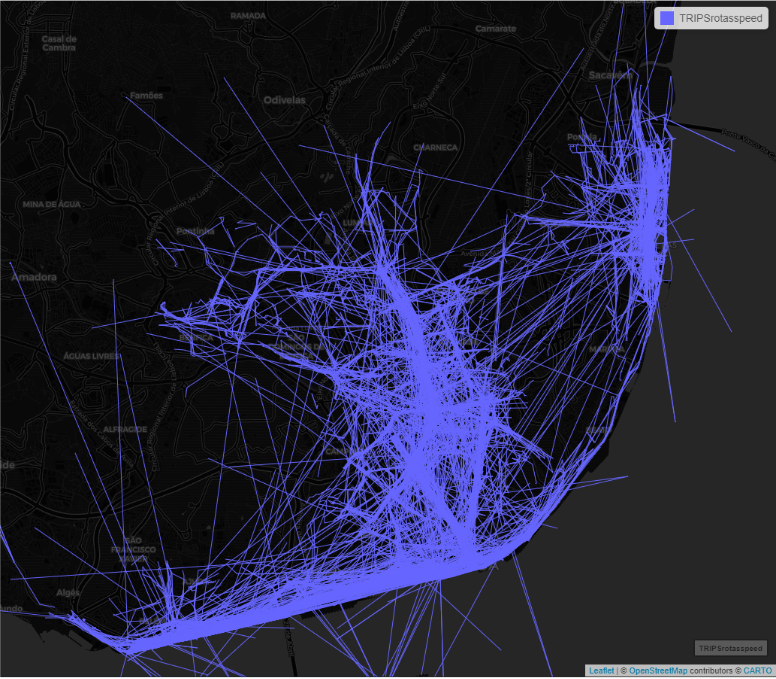
\includegraphics[width=6.25in,height=\textheight]{images/clipboard-2086563605.png}

}

\caption{E-Scooter trip data in Lisbon. How to deal with it?}

\end{figure}%

Knowing how to get, treat and analyze complex datasets with the
up-to-date technologies is extremely relevant for academia, policy
makers and start-ups, since it allows them to:

\begin{enumerate}
\def\labelenumi{\arabic{enumi}.}
\item
  acquire critical view on urban mobility based on data;
\item
  spatially identify locations in the city that require policy
  priorities;
\item
  and improve the efficiency of data analysis processes.
\end{enumerate}

\subsection*{Why R and GIS}\label{why-r-and-gis}
\addcontentsline{toc}{subsection}{Why R and GIS}

Most academic programs focus on teaching modelling and deep analysis of
data. However, there is a need to learn how to explore and prepare a
dataset for modelling. The use of \textbf{programming and GIS}
techniques have enormous advantages, including their flexibility;
reproducibility; and transparency and understanding the step-by-step
process.

The use of GIS techniques in transportation is, traditionally, not
considered in transportation learning programs, despite being of
enormous relevance when doing accessibility analysis or reeling with
georreferenced transportation data, such as bike sharing route trips'
datasets, origin-destination flows datasets, home/work locations, GTFS
public transit data, and so on. There is a need to learn how to locate
these open datasets, how to explore them and how to integrate them into
transportation and urban analysis. Additionally, the use of open source
software and datasets allows researchers to perform methods that are
reproducible and transparent.

\subsubsection*{TLDR}\label{tldr}
\addcontentsline{toc}{subsubsection}{TLDR}

\begin{itemize}
\item
  Open-source tools widely used in data analytics and spatial analysis
\item
  Flexibility and reproducibility in data manipulation and visualization
\item
  Critical for urban mobility and transportation research, with spatial
  relevance
\item
  Large transportation datasets are becoming increasingly common
\end{itemize}

\section{Course objectives}\label{course-objectives}

\subsection*{Introduce R Programming
Basics}\label{introduce-r-programming-basics}
\addcontentsline{toc}{subsection}{Introduce R Programming Basics}

\begin{itemize}
\item
  Equip participants with foundational skills in R programming
\item
  Emphasize reproducible research practices to ensure transparency and
  replicability in analyses
\end{itemize}

\subsection*{Teach Data Manipulation
Techniques}\label{teach-data-manipulation-techniques}
\addcontentsline{toc}{subsection}{Teach Data Manipulation Techniques}

\begin{itemize}
\item
  Use key R packages for data cleaning, manipulation, and summarization
  of datasets
\item
  Enable participants to efficiently handle large and complex
  transportation datasets
\end{itemize}

\subsection*{Spatial Data
Visualization}\label{spatial-data-visualization}
\addcontentsline{toc}{subsection}{Spatial Data Visualization}

\begin{itemize}
\item
  Introduce methods for quick and effective spatial data visualization
  using R and GIS tools
\item
  Provide hands-on experience with creating interactive maps and
  visualizations
\end{itemize}

\subsection*{Perform Basic Spatial
Analysis}\label{perform-basic-spatial-analysis}
\addcontentsline{toc}{subsection}{Perform Basic Spatial Analysis}

\begin{itemize}
\item
  Teach participants how to perform spatial analysis of transportation
  datasets using GIS techniques with R
\item
  Cover practical applications such as georeferencing data,
  accessibility analysis, and routing ODs
\item
  Utilize real-world transportation data for practical, hands-on
  learning
\end{itemize}

\section{Target audience}\label{target-audience}

\begin{itemize}
\item
  Ph.D.~candidates from DTN and other researchers
\item
  Policy makers and practitioners in urban mobility
\item
  Beginners to intermediate R users, no prior experience needed
\end{itemize}

\section{Recommended readings}\label{recommended-readings}

\begin{itemize}
\tightlist
\item
  Engel, Claudia A (2023)
  \href{https://cengel.github.io/R-intro/}{Introduction to R}
\item
  Lovelace, Robin, Nowosad, Jakub \& Muenchow, Johannes (2023)
  \href{https://geocompr.robinlovelace.net/}{Geocomputation with R}
\item
  Pereira, Rafael H. M. \& Herszenhut, Daniel (2023)
  \href{https://ipeagit.github.io/intro_access_book/index.en.html}{Introduction
  to urban accessibility: a practical guide with R}. Ipea - Institute of
  Applied Economic Research
\end{itemize}

\bookmarksetup{startatroot}

\chapter{Course Structure}\label{course-structure}

The course consists of an in-person 2-day course, taking place during
the EIT DTN Annual Meeting on the \textbf{19th and 20th September 2024}.

The first day will focus on learning the basics of R programming and how
to treat and explore datasets. The second day will focus on analyzing
spatial datasets, and routing origins to destinations.

\section{Day 1}\label{day-1}

\subsection*{Morning}\label{morning}
\addcontentsline{toc}{subsection}{Morning}

We will start by a brief introduction to this course, followed by an
introduction to programming techniques and data structures.

Then, we will install R and RStudio, and and the required R packages for
this course, as in \href{software.qmd}{Software} section.

After having everything setup, we will start with the
\href{r-basics.qmd}{R basics}, with examples and exercises.

\subsection*{Afternoon}\label{afternoon}
\addcontentsline{toc}{subsection}{Afternoon}

In the afternoon, we will focus on \href{data-manipulation.qmd}{data
manipulation}, using the dplyr package to select, filter, left-join,
group and summarize datasets.

Then, we will \href{spatial-data.qmd}{introduce GIS and spatial data},
learning how to importing and visualize vector data.

Finally, we will learn how to create cool
\href{interactive-maps.qmd}{interactive maps} using mapview and R
markdown.

\section{Day 2}\label{day-2}

\subsection*{Morning}\label{morning-1}
\addcontentsline{toc}{subsection}{Morning}

We will start the day by estimating the different types of
\href{centroids.qmd}{centroids of transport zones}.

After this, the natural next step is to create
\href{desire-lines.qmd}{desire lines} from orgins and destinations of
the transport zones.

We will then learn how to estimate \href{distances.qmd}{euclidean and
routing distances} for the desire-lines, using transport networks.

\subsection*{Afternoon}\label{afternoon-1}
\addcontentsline{toc}{subsection}{Afternoon}

In the second afternoon, we will briefly learn where to find and extract
\href{open-data.qmd}{open transportation data}, such as OpenStreetMap
and GTFS.

Then, we will learn how to perform \href{r5r.qmd}{accessibility
analysis}, using the r5r package.

And finally, to wrap up all this topics, we will have a group exercise
using other complex datasets, where you will apply the knowledge learned
during the course.

\bookmarksetup{startatroot}

\chapter{Detailed schedule (TBC)}\label{detailed-schedule-tbc}

\begin{longtable}[]{@{}
  >{\raggedright\arraybackslash}p{(\columnwidth - 2\tabcolsep) * \real{0.2778}}
  >{\raggedright\arraybackslash}p{(\columnwidth - 2\tabcolsep) * \real{0.7222}}@{}}
\toprule\noalign{}
\begin{minipage}[b]{\linewidth}\raggedright
Day 1
\end{minipage} & \begin{minipage}[b]{\linewidth}\raggedright
\end{minipage} \\
\midrule\noalign{}
\endhead
\bottomrule\noalign{}
\endlastfoot
9.30 & Introductions and Presentation of the course contents \\
10.00 & Introduction to programming techniques and data structures \\
10.30 & Introduction to R and RStudio: hands-on to install software and
main packages \\
11.00 & \emph{Coffee break} \\
11.15 & (cont.) \\
11.30 & R basics: examples and exercises \\
& \\
12.30 & \emph{Lunch break} \\
& \\
13.30 & Data manipulation: examples and exercises (select, filter,
left-join, group and summarize, using~dplyr package) \\
15.30 & \emph{Coffee break} \\
15.45 & Introduction to GIS and spatial data: import create vector
data \\
16.30 & View and export interactive maps \\
17.00 & \emph{End of day 1} \\
\end{longtable}

\begin{longtable}[]{@{}
  >{\raggedright\arraybackslash}p{(\columnwidth - 2\tabcolsep) * \real{0.2778}}
  >{\raggedright\arraybackslash}p{(\columnwidth - 2\tabcolsep) * \real{0.7222}}@{}}
\toprule\noalign{}
\begin{minipage}[b]{\linewidth}\raggedright
Day 2
\end{minipage} & \begin{minipage}[b]{\linewidth}\raggedright
\end{minipage} \\
\midrule\noalign{}
\endhead
\bottomrule\noalign{}
\endlastfoot
9.30 & Centroids of transport zones \\
10.15 & Desire-lines from OD pairs and transport zones \\
11.00 & \emph{Coffee break} \\
11.15 & (cont.) \\
11.30 & Euclidean and routing distances with sf and r5r \\
& \\
12.30 & \emph{Lunch break} \\
& \\
13.30 & Open Transportation data: where to find it (OSM and GTFS) \\
14.00 & Accessibility analysis with r5r \\
16.00 & \emph{Coffee break} \\
16.15 & Using you data: manipulation and spatial analysis methods and
further applications \\
16.45 & Survey and feedback from participants \\
17.00 & \emph{End of day 2} \\
\end{longtable}

\bookmarksetup{startatroot}

\chapter{Location}\label{location}

The course will take place at Campus Sterre, Building S8, room 2.4.

\begin{Shaded}
\begin{Highlighting}[]
\NormalTok{Campus\_S8\_coord }\OtherTok{=} \FunctionTok{c}\NormalTok{(}\FloatTok{3.7105372}\NormalTok{, }\FloatTok{51.0241258}\NormalTok{)}
\NormalTok{Campus\_S8 }\OtherTok{=}\NormalTok{ sf}\SpecialCharTok{::}\FunctionTok{st\_sfc}\NormalTok{(sf}\SpecialCharTok{::}\FunctionTok{st\_point}\NormalTok{(Campus\_S8\_coord)) }\CommentTok{\# create point}
\NormalTok{Campus\_S8 }\OtherTok{=}\NormalTok{ sf}\SpecialCharTok{::}\FunctionTok{st\_as\_sf}\NormalTok{(Campus\_S8, }\AttributeTok{crs =} \DecValTok{4326}\NormalTok{) }\CommentTok{\# assign crs}

\NormalTok{mapview}\SpecialCharTok{::}\FunctionTok{mapview}\NormalTok{(Campus\_S8, }\AttributeTok{map.types =} \StringTok{"OpenStreetMap"}\NormalTok{) }\CommentTok{\# quick map view}
\end{Highlighting}
\end{Shaded}

\includegraphics{structure_files/figure-pdf/unnamed-chunk-1-1.png}

\bookmarksetup{startatroot}

\chapter{Resources}\label{resources}

\begin{itemize}
\item
  You laptop, with any OS
\item
  Github repository with all the materials (data, code and guidelines)
\item
  Survey datasets, school locations and public transport operator
  datasets
\end{itemize}

\part{\textbf{Day 1}}

\chapter{Software}\label{software}

In this chapter we will guide you through the installation of R, RStudio
and the packages you will need for this course.

\textbf{R} and \textbf{RStudio}\footnote{We will use RStudio, although
  if you already use other studio such as VScode, that's also fine.} are
separate downloads.

\section{R}\label{r}

You will need \textbf{R} installed on your computer. \textbf{R stats}
(how it is also known) is a programming language and free software
environment for statistical computing and graphics supported by the R
Foundation for Statistical Computing.

The download links live at \href{https://cran.r-project.org/}{The
Comprehensive R Archive Network} (aka CRAN). The most recent version is
\texttt{4.4.1}, but you can use \texttt{\textgreater{}=\ 4.1.x} if you
already have it installed.

\subsection{Windows}

\href{https://cran.r-project.org/bin/windows/base/R-4.4.1-win.exe}{Download
R-4.4.1 for Windows} and run the executable file.

You will also need to install Rtools, which is a collection of tools
necessary to build R packages in Windows.

\subsection{Mac}

\href{https://cran.r-project.org/}{Download R-4.4.1 for MacOX}. You will
have to choose between the arm64 or the x86-64 version.

Download the \texttt{.pkg} file and install it as usual.

\subsection{Ubuntu}

\begin{quote}
These are instructions for Ubuntu. If you use other linux distribution,
please follow the instructions on
\href{https://cran.r-project.org/bin/linux/}{The Comprehensive R Archive
Network - CRAN}.
\end{quote}

You can look for R in the Ubuntu \textbf{Software Center} or install it
via the terminal:

\begin{Shaded}
\begin{Highlighting}[]
\CommentTok{\# sudo apt update \&\& sudo apt upgrade {-}y}
\FunctionTok{sudo}\NormalTok{ apt install r{-}base}
\end{Highlighting}
\end{Shaded}

\textbf{Or}, if you prefer, you can install the latest version of R from
CRAN:

\begin{Shaded}
\begin{Highlighting}[]
\CommentTok{\# update indices}
\FunctionTok{sudo}\NormalTok{ apt update }\AttributeTok{{-}qq}
\CommentTok{\# install two helper packages we need}
\FunctionTok{sudo}\NormalTok{ apt install }\AttributeTok{{-}{-}no{-}install{-}recommends}\NormalTok{ software{-}properties{-}common dirmngr}
\CommentTok{\# add the signing key (by Michael Rutter) for these repos}
\FunctionTok{wget} \AttributeTok{{-}qO{-}}\NormalTok{ https://cloud.r{-}project.org/bin/linux/ubuntu/marutter\_pubkey.asc }\KeywordTok{|} \FunctionTok{sudo}\NormalTok{ tee }\AttributeTok{{-}a}\NormalTok{ /etc/apt/trusted.gpg.d/cran\_ubuntu\_key.asc}
\CommentTok{\# add the R 4.0 repo from CRAN {-}{-} adjust \textquotesingle{}focal\textquotesingle{} to \textquotesingle{}groovy\textquotesingle{} or \textquotesingle{}bionic\textquotesingle{} as needed}
\FunctionTok{sudo}\NormalTok{ add{-}apt{-}repository }\StringTok{"deb https://cloud.r{-}project.org/bin/linux/ubuntu }\VariableTok{$(}\ExtensionTok{lsb\_release} \AttributeTok{{-}cs}\VariableTok{)}\StringTok{{-}cran40/"}
\end{Highlighting}
\end{Shaded}

Then run:

\begin{Shaded}
\begin{Highlighting}[]
\FunctionTok{sudo}\NormalTok{ apt install r{-}base r{-}base{-}core r{-}recommended r{-}base{-}dev}
\end{Highlighting}
\end{Shaded}

{[}Optional{]} To keep up-to-date r version and packages, you can follow
the instructions at \href{https://eddelbuettel.github.io/r2u/}{r2u}

After this installation, you don't need to open R base. Please proceed
to install RStudio.

\section{RStudio}\label{rstudio}

RStudio Desktop is an integrated development environment (IDE) for R. It
includes a console, syntax-highlighting editor that supports direct code
execution, as well as tools for plotting, history, debugging and
workspace management.

RStudio is available for free download from
\href{https://posit.co/download/rstudio-desktop/}{Posit RStudio}.

\subsection{Windows 10/11}

\href{https://download1.rstudio.org/electron/windows/RStudio-2024.04.2-764.exe}{Download
RStudio 2024.04} and run the executable file.

\subsection{MacOS}

\href{https://download1.rstudio.org/electron/macos/RStudio-2024.04.2-764.dmg}{Download
RStudio 2024.04} and install it as usual.

\subsection{Ubuntu}

\begin{quote}
These are instructions for Ubuntu \textbf{22} / Debian 12. If you use
other linux distribution, please follow the instructions on
\href{https://posit.co/download/rstudio-desktop/}{Posit RStudio}.
\end{quote}

Install it via the terminal:

\begin{Shaded}
\begin{Highlighting}[]
\FunctionTok{sudo}\NormalTok{ apt install libssl{-}dev libclang{-}dev}
\FunctionTok{wget}\NormalTok{ https://download1.rstudio.org/electron/jammy/amd64/rstudio{-}2024.04.2{-}764{-}amd64.deb}
\FunctionTok{sudo}\NormalTok{ dpkg }\AttributeTok{{-}i}\NormalTok{ rstudio}\PreprocessorTok{*}
\FunctionTok{rm} \AttributeTok{{-}v}\NormalTok{ rstudio}\PreprocessorTok{*}
\end{Highlighting}
\end{Shaded}

If you already use Ubuntu \textbf{24}, please check and replace the
correct url from \href{https://dailies.rstudio.com/}{RStudio Dailies}

\section{R packages}\label{r-packages}

You will need to install some packages to work with the data and scripts
in this course.

You can install them in RStudio by searching for them in the
\textbf{Packages} tab:

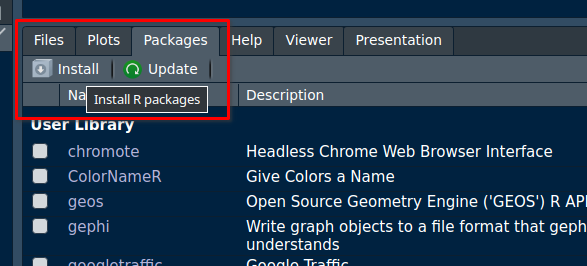
\includegraphics{images/clipboard-3443685728.png}

\textbf{or} by running the following code in the console:

\begin{Shaded}
\begin{Highlighting}[]
\FunctionTok{install.packages}\NormalTok{(}\StringTok{"tidyverse"}\NormalTok{)}
\FunctionTok{install.packages}\NormalTok{(}\StringTok{"readxl"}\NormalTok{)}

\FunctionTok{install.packages}\NormalTok{(}\StringTok{"sf"}\NormalTok{)}
\FunctionTok{install.packages}\NormalTok{(}\StringTok{"mapview"}\NormalTok{)}
\FunctionTok{install.packages}\NormalTok{(}\StringTok{"rmarkdown"}\NormalTok{)}
\FunctionTok{install.packages}\NormalTok{(}\StringTok{"centr"}\NormalTok{)}
\FunctionTok{install.packages}\NormalTok{(}\StringTok{"od"}\NormalTok{)}

\FunctionTok{install.packages}\NormalTok{(}\FunctionTok{c}\NormalTok{(}\StringTok{"remotes"}\NormalTok{, }\StringTok{"devtools"}\NormalTok{, }\StringTok{"usethis"}\NormalTok{)) }\CommentTok{\# optional}
\FunctionTok{install.packages}\NormalTok{(}\StringTok{"osmextract"}\NormalTok{) }\CommentTok{\# optional}
\FunctionTok{install.packages}\NormalTok{(}\StringTok{"stplanr"}\NormalTok{) }\CommentTok{\# optional}
\end{Highlighting}
\end{Shaded}

\section{r5r}\label{r5r}

The workshop~\textbf{``A crash course on urban accessibility with R''}
uses a few R packages that need to be installed on your machine. The
simplest way to do this is running the code below. This might take a few
minutes if this is the first time you install these packages.

\begin{Shaded}
\begin{Highlighting}[]
\NormalTok{pkgs }\OtherTok{=} \FunctionTok{c}\NormalTok{(}\StringTok{"r5r"}\NormalTok{, }\StringTok{"accessibility"}\NormalTok{, }\StringTok{"rJavaEnv"}\NormalTok{, }\StringTok{"h3jsr"}\NormalTok{)}

\FunctionTok{install.packages}\NormalTok{(pkgs)}
\end{Highlighting}
\end{Shaded}

\subsection{Java Development Kit}\label{java-development-kit}

To use the \texttt{\{r5r\}} package (version v2.0 or higher), you will
need to have \emph{Java Development Kit (JDK) 21} installed on your
computer. There are numerous open-source JDK implementations. The
easiest way to install JDK is using the new
\href{https://www.ekotov.pro/rJavaEnv/}{\{rJavaEnv\}} package in R.

\begin{Shaded}
\begin{Highlighting}[]
\CommentTok{\# check version of Java currently installed (if any) }
\NormalTok{rJavaEnv}\SpecialCharTok{::}\FunctionTok{java\_check\_version\_rjava}\NormalTok{()}

\DocumentationTok{\#\# if this is the first time you use \{rJavaEnv\}, you might need to run this code}
\DocumentationTok{\#\# below to consent the installation of Java.}
\CommentTok{\# rJavaEnv::rje\_consent(provided = TRUE)}

\CommentTok{\# install Java 21}
\NormalTok{rJavaEnv}\SpecialCharTok{::}\FunctionTok{java\_quick\_install}\NormalTok{(}
  \AttributeTok{version =} \DecValTok{21}\NormalTok{,}
  \AttributeTok{distribution =} \StringTok{\textquotesingle{}Corretto\textquotesingle{}}\NormalTok{)}

\CommentTok{\# check if Java was successfully installed}
\NormalTok{rJavaEnv}\SpecialCharTok{::}\FunctionTok{java\_check\_version\_rjava}\NormalTok{()}
\end{Highlighting}
\end{Shaded}

\textbf{Alternatively}, you can manually download and install JDK 21.

\subsection{Windows and MacOS}

Go to \href{https://jdk.java.net/archive/}{Java Development Kit 21},
download the latest 21 build corresponding to your operating system and
run the executable file.

\subsection{Ubuntu}

Install it via the terminal:

\begin{Shaded}
\begin{Highlighting}[]
\FunctionTok{sudo}\NormalTok{ apt install }\AttributeTok{{-}y}\NormalTok{ openjdk{-}21{-}jdk openjdk{-}21{-}jre}
\ExtensionTok{java} \AttributeTok{{-}version}
\end{Highlighting}
\end{Shaded}

\chapter{R basics}\label{r-basics}

In this chapter we will introduce to the R basics and some exercises to
get familiar to how R works.

\section{Math operations}\label{math-operations}

\subsection{Sum}\label{sum}

\begin{Shaded}
\begin{Highlighting}[]
\DecValTok{1}\SpecialCharTok{+}\DecValTok{1}
\end{Highlighting}
\end{Shaded}

\begin{verbatim}
[1] 2
\end{verbatim}

\subsection{Subtraction}\label{subtraction}

\begin{Shaded}
\begin{Highlighting}[]
\DecValTok{5{-}2}
\end{Highlighting}
\end{Shaded}

\begin{verbatim}
[1] 3
\end{verbatim}

\subsection{Multiplication}\label{multiplication}

\begin{Shaded}
\begin{Highlighting}[]
\DecValTok{2}\SpecialCharTok{*}\DecValTok{2}
\end{Highlighting}
\end{Shaded}

\begin{verbatim}
[1] 4
\end{verbatim}

\subsection{Division}\label{division}

\begin{Shaded}
\begin{Highlighting}[]
\DecValTok{8}\SpecialCharTok{/}\DecValTok{2}
\end{Highlighting}
\end{Shaded}

\begin{verbatim}
[1] 4
\end{verbatim}

\subsection{Round the number}\label{round-the-number}

\begin{Shaded}
\begin{Highlighting}[]
\FunctionTok{round}\NormalTok{(}\FloatTok{3.14}\NormalTok{)}
\end{Highlighting}
\end{Shaded}

\begin{verbatim}
[1] 3
\end{verbatim}

\begin{Shaded}
\begin{Highlighting}[]
\FunctionTok{round}\NormalTok{(}\FloatTok{3.14}\NormalTok{, }\DecValTok{1}\NormalTok{) }\CommentTok{\# The "1" indicates to round it up to 1 decimal digit.}
\end{Highlighting}
\end{Shaded}

\begin{verbatim}
[1] 3.1
\end{verbatim}

You can use help \texttt{?round} in the console to see the description
of the function, and the default arguments.

\section{Basic shortpaths}\label{basic-shortpaths}

\subsection{Perform Combinations}\label{perform-combinations}

\begin{Shaded}
\begin{Highlighting}[]
\FunctionTok{c}\NormalTok{(}\DecValTok{1}\NormalTok{, }\DecValTok{2}\NormalTok{, }\DecValTok{3}\NormalTok{)}
\end{Highlighting}
\end{Shaded}

\begin{verbatim}
[1] 1 2 3
\end{verbatim}

\begin{Shaded}
\begin{Highlighting}[]
\FunctionTok{c}\NormalTok{(}\DecValTok{1}\SpecialCharTok{:}\DecValTok{3}\NormalTok{) }\CommentTok{\# The ":" indicates a range between the first and second numbers. }
\end{Highlighting}
\end{Shaded}

\begin{verbatim}
[1] 1 2 3
\end{verbatim}

\subsection{\texorpdfstring{Create a comment with
\texttt{ctrl\ +\ shift\ +\ m}}{Create a comment with ctrl + shift + m}}\label{create-a-comment-with-ctrl-shift-m}

\begin{Shaded}
\begin{Highlighting}[]
\CommentTok{\# Comments help you organize your code. The software will not run the comment. }
\end{Highlighting}
\end{Shaded}

\subsection{Create a table}\label{create-a-table}

A simple table with the number of trips by car, PT, walking, and cycling
in a hypothetical street segment at a certain period.

\textbf{Define variables}

\begin{Shaded}
\begin{Highlighting}[]
\NormalTok{modes }\OtherTok{\textless{}{-}} \FunctionTok{c}\NormalTok{(}\StringTok{"car"}\NormalTok{, }\StringTok{"PT"}\NormalTok{, }\StringTok{"walking"}\NormalTok{, }\StringTok{"cycling"}\NormalTok{) }\CommentTok{\# you can use "=" or "\textless{}{-}"}
\NormalTok{Trips }\OtherTok{=} \FunctionTok{c}\NormalTok{(}\DecValTok{200}\NormalTok{, }\DecValTok{50}\NormalTok{, }\DecValTok{300}\NormalTok{, }\DecValTok{150}\NormalTok{) }\CommentTok{\# uppercase letters modify}
\end{Highlighting}
\end{Shaded}

\textbf{Join the variables to create a table}

\begin{Shaded}
\begin{Highlighting}[]
\NormalTok{table\_example }\OtherTok{=} \FunctionTok{data.frame}\NormalTok{(modes, Trips)}
\end{Highlighting}
\end{Shaded}

\textbf{Take a look at the table}

Visualize the table by clicking on the ``Data'' in the ``Environment''
page or use :

\begin{Shaded}
\begin{Highlighting}[]
\FunctionTok{View}\NormalTok{(table\_example)}
\end{Highlighting}
\end{Shaded}

\section{Practical exercise}\label{practical-exercise}

\textbf{Dataset:} the number of trips between all municipalities in the
Lisbon Metropolitan Area, Portugal (INE 2018).

\subsection{Import dataset}\label{import-dataset}

You can click directly in the file under the ``Files'' pan, or:

\begin{Shaded}
\begin{Highlighting}[]
\NormalTok{data }\OtherTok{=} \FunctionTok{readRDS}\NormalTok{(}\StringTok{"data/TRIPSmode.Rds"}\NormalTok{)}
\end{Highlighting}
\end{Shaded}

\begin{tcolorbox}[enhanced jigsaw, breakable, left=2mm, colframe=quarto-callout-tip-color-frame, leftrule=.75mm, bottomrule=.15mm, arc=.35mm, rightrule=.15mm, colback=white, opacityback=0, toprule=.15mm]
\begin{minipage}[t]{5.5mm}
\textcolor{quarto-callout-tip-color}{\faLightbulb}
\end{minipage}%
\begin{minipage}[t]{\textwidth - 5.5mm}

After you type \texttt{"} you can use \texttt{tab} to navigate between
folders and files and \texttt{enter} to autocomplete.

\end{minipage}%
\end{tcolorbox}

\subsection{Take a first look at the
data}\label{take-a-first-look-at-the-data}

\textbf{Summary statistics}

\begin{Shaded}
\begin{Highlighting}[]
\FunctionTok{summary}\NormalTok{(data)}
\end{Highlighting}
\end{Shaded}

\begin{verbatim}
    Origin          Destination            Total             Walk       
 Length:315         Length:315         Min.   :     7   Min.   :     0  
 Class :character   Class :character   1st Qu.:   330   1st Qu.:     0  
 Mode  :character   Mode  :character   Median :  1090   Median :     0  
                                       Mean   : 16825   Mean   :  4033  
                                       3rd Qu.:  5374   3rd Qu.:     0  
                                       Max.   :875144   Max.   :306289  
      Bike              Car            PTransit            Other        
 Min.   :   0.00   Min.   :     0   Min.   :     0.0   Min.   :    0.0  
 1st Qu.:   0.00   1st Qu.:   263   1st Qu.:     5.0   1st Qu.:    0.0  
 Median :   0.00   Median :   913   Median :   134.0   Median :    0.0  
 Mean   :  80.19   Mean   :  9956   Mean   :  2602.6   Mean   :  152.4  
 3rd Qu.:   0.00   3rd Qu.:  4408   3rd Qu.:   975.5   3rd Qu.:   62.5  
 Max.   :5362.00   Max.   :349815   Max.   :202428.0   Max.   :11647.0  
\end{verbatim}

\textbf{Check the structure of the data}

\begin{Shaded}
\begin{Highlighting}[]
\FunctionTok{str}\NormalTok{(data)}
\end{Highlighting}
\end{Shaded}

\begin{verbatim}
'data.frame':   315 obs. of  8 variables:
 $ Origin     : chr  "Alcochete" "Alcochete" "Alcochete" "Alcochete" ...
 $ Destination: chr  "Alcochete" "Almada" "Amadora" "Barreiro" ...
 $ Total      : num  20478 567 188 867 114 ...
 $ Walk       : num  6833 0 0 0 0 ...
 $ Bike       : num  320 0 0 0 0 0 0 0 91 0 ...
 $ Car        : num  12484 353 107 861 114 ...
 $ PTransit   : num  833 0 81 5 0 ...
 $ Other      : num  7 214 0 0 0 0 0 0 0 0 ...
\end{verbatim}

\textbf{Check the first values of each variable}

\begin{Shaded}
\begin{Highlighting}[]
\NormalTok{data}
\end{Highlighting}
\end{Shaded}

\begin{Shaded}
\begin{Highlighting}[]
\FunctionTok{head}\NormalTok{(data, }\DecValTok{3}\NormalTok{) }\CommentTok{\# first 3 values}
\end{Highlighting}
\end{Shaded}

\begin{verbatim}
     Origin Destination Total Walk Bike   Car PTransit Other
1 Alcochete   Alcochete 20478 6833  320 12484      833     7
2 Alcochete      Almada   567    0    0   353        0   214
3 Alcochete     Amadora   188    0    0   107       81     0
\end{verbatim}

\textbf{Check the number of rows (observations) and columns (variables)}

\begin{Shaded}
\begin{Highlighting}[]
\FunctionTok{nrow}\NormalTok{(data)}
\end{Highlighting}
\end{Shaded}

\begin{verbatim}
[1] 315
\end{verbatim}

\begin{Shaded}
\begin{Highlighting}[]
\FunctionTok{ncol}\NormalTok{(data)}
\end{Highlighting}
\end{Shaded}

\begin{verbatim}
[1] 8
\end{verbatim}

\textbf{Open the dataset}

\begin{Shaded}
\begin{Highlighting}[]
\FunctionTok{View}\NormalTok{(data)}
\end{Highlighting}
\end{Shaded}

\subsection{Explore the data}\label{explore-the-data}

\textbf{Check the total number of trips}

Use \texttt{\$} to select a variable of the data

\begin{Shaded}
\begin{Highlighting}[]
\FunctionTok{sum}\NormalTok{(data}\SpecialCharTok{$}\NormalTok{Total)}
\end{Highlighting}
\end{Shaded}

\begin{verbatim}
[1] 5299853
\end{verbatim}

\textbf{Percentage of car trips related to the total}

\begin{Shaded}
\begin{Highlighting}[]
\FunctionTok{sum}\NormalTok{(data}\SpecialCharTok{$}\NormalTok{Car)}\SpecialCharTok{/}\FunctionTok{sum}\NormalTok{(data}\SpecialCharTok{$}\NormalTok{Total) }\SpecialCharTok{*} \DecValTok{100}
\end{Highlighting}
\end{Shaded}

\begin{verbatim}
[1] 59.17638
\end{verbatim}

\textbf{Percentage of active trips related to the total}

\begin{Shaded}
\begin{Highlighting}[]
\NormalTok{(}\FunctionTok{sum}\NormalTok{(data}\SpecialCharTok{$}\NormalTok{Walk) }\SpecialCharTok{+} \FunctionTok{sum}\NormalTok{(data}\SpecialCharTok{$}\NormalTok{Bike)) }\SpecialCharTok{/} \FunctionTok{sum}\NormalTok{(data}\SpecialCharTok{$}\NormalTok{Total) }\SpecialCharTok{*} \DecValTok{100}
\end{Highlighting}
\end{Shaded}

\begin{verbatim}
[1] 24.44883
\end{verbatim}

\subsection{Modify original data}\label{modify-original-data}

\textbf{Create a column with the sum of the number of trips for active
modes}

\begin{Shaded}
\begin{Highlighting}[]
\NormalTok{data}\SpecialCharTok{$}\NormalTok{Active }\OtherTok{=}\NormalTok{ data}\SpecialCharTok{$}\NormalTok{Walk }\SpecialCharTok{+}\NormalTok{ data}\SpecialCharTok{$}\NormalTok{Bike}
\end{Highlighting}
\end{Shaded}

\textbf{Filter by condition (create new tables)}

Filter trips only with origin from Lisbon

\begin{Shaded}
\begin{Highlighting}[]
\NormalTok{data\_Lisbon }\OtherTok{=}\NormalTok{ data[data}\SpecialCharTok{$}\NormalTok{Origin }\SpecialCharTok{==} \StringTok{"Lisboa"}\NormalTok{,]}
\end{Highlighting}
\end{Shaded}

Filter trips with origin \textbf{different} from Lisbon

\begin{Shaded}
\begin{Highlighting}[]
\NormalTok{data\_out\_Lisbon }\OtherTok{=}\NormalTok{ data[data}\SpecialCharTok{$}\NormalTok{Origin }\SpecialCharTok{!=} \StringTok{"Lisboa"}\NormalTok{,]}
\end{Highlighting}
\end{Shaded}

Filter trips with origin \textbf{and} destination in Lisbon

\begin{Shaded}
\begin{Highlighting}[]
\NormalTok{data\_in\_Out\_Lisbon }\OtherTok{=}\NormalTok{ data[data}\SpecialCharTok{$}\NormalTok{Origin }\SpecialCharTok{==} \StringTok{"Lisboa"} \SpecialCharTok{\&}\NormalTok{ data}\SpecialCharTok{$}\NormalTok{Destination }\SpecialCharTok{==} \StringTok{"Lisboa"}\NormalTok{,]}
\end{Highlighting}
\end{Shaded}

\textbf{Remove a column}

Look at the first row

\begin{Shaded}
\begin{Highlighting}[]
\NormalTok{data[}\DecValTok{1}\NormalTok{,] }\CommentTok{\#rows and columns start from 1}
\end{Highlighting}
\end{Shaded}

\begin{verbatim}
     Origin Destination Total Walk Bike   Car PTransit Other Active
1 Alcochete   Alcochete 20478 6833  320 12484      833     7   7153
\end{verbatim}

Look at first row and column

\begin{Shaded}
\begin{Highlighting}[]
\NormalTok{data[}\DecValTok{1}\NormalTok{,}\DecValTok{1}\NormalTok{]}
\end{Highlighting}
\end{Shaded}

\begin{verbatim}
[1] "Alcochete"
\end{verbatim}

Remove the first column

\begin{Shaded}
\begin{Highlighting}[]
\NormalTok{data }\OtherTok{=}\NormalTok{ data[ ,}\SpecialCharTok{{-}}\DecValTok{1}\NormalTok{] }\CommentTok{\#first column}
\end{Highlighting}
\end{Shaded}

\textbf{Create a table only with origin, destination and walking trips}

There are many ways to do the same operation.

\begin{Shaded}
\begin{Highlighting}[]
\FunctionTok{names}\NormalTok{(data)}
\end{Highlighting}
\end{Shaded}

\begin{verbatim}
[1] "Destination" "Total"       "Walk"        "Bike"        "Car"        
[6] "PTransit"    "Other"       "Active"     
\end{verbatim}

\begin{Shaded}
\begin{Highlighting}[]
\NormalTok{data\_walk2 }\OtherTok{=}\NormalTok{ data[ ,}\FunctionTok{c}\NormalTok{(}\DecValTok{1}\NormalTok{,}\DecValTok{2}\NormalTok{,}\DecValTok{4}\NormalTok{)]}
\end{Highlighting}
\end{Shaded}

\begin{Shaded}
\begin{Highlighting}[]
\NormalTok{data\_walk3 }\OtherTok{=}\NormalTok{ data[ ,}\SpecialCharTok{{-}}\FunctionTok{c}\NormalTok{(}\DecValTok{3}\NormalTok{,}\DecValTok{5}\SpecialCharTok{:}\DecValTok{9}\NormalTok{)]}
\end{Highlighting}
\end{Shaded}

\subsection{Export data}\label{export-data}

Save data in \textbf{.csv} and \textbf{.Rds}

\begin{Shaded}
\begin{Highlighting}[]
\FunctionTok{write.csv}\NormalTok{(data, }\StringTok{\textquotesingle{}data/dataset.csv\textquotesingle{}}\NormalTok{, }\AttributeTok{row.names =} \ConstantTok{FALSE}\NormalTok{)}
\FunctionTok{saveRDS}\NormalTok{(data, }\StringTok{\textquotesingle{}data/dataset.Rds\textquotesingle{}}\NormalTok{) }\CommentTok{\#Choose a different file. }
\end{Highlighting}
\end{Shaded}

\subsection{Import data}\label{import-data}

\begin{Shaded}
\begin{Highlighting}[]
\NormalTok{csv\_file }\OtherTok{=} \FunctionTok{read.csv}\NormalTok{(}\StringTok{"data/dataset.csv"}\NormalTok{)}
\NormalTok{rds\_file }\OtherTok{=} \FunctionTok{readRDS}\NormalTok{(}\StringTok{"data/dataset.Rds"}\NormalTok{)}
\end{Highlighting}
\end{Shaded}

\chapter{Data manipulation}\label{data-manipulation}

In this chapter we will use some very useful \texttt{dplyr} functions to
handle and manipulate data.

You can load the \texttt{dplyr} package directly, or load the entire
tidy universe (\texttt{tidyverse}).

\begin{Shaded}
\begin{Highlighting}[]
\CommentTok{\# library(tidyverse)}
\FunctionTok{library}\NormalTok{(dplyr)}
\end{Highlighting}
\end{Shaded}

Using the same dataset as in
\href{https://u-shift.github.io/EITcourse/r-basics.html}{R basics} but
with slightly differences\footnote{This dataset includes the number of
  trips with origin in each neighborhood, divided by mode of transport,
  and inter or intra municipal trips.}.

We will do the same operations but in a simplified way.

\begin{Shaded}
\begin{Highlighting}[]
\NormalTok{TRIPS }\OtherTok{=} \FunctionTok{readRDS}\NormalTok{(}\StringTok{"data/TRIPSorigin.Rds"}\NormalTok{)}
\end{Highlighting}
\end{Shaded}

\begin{tcolorbox}[enhanced jigsaw, left=2mm, toprule=.15mm, toptitle=1mm, leftrule=.75mm, titlerule=0mm, colback=white, opacityback=0, opacitybacktitle=0.6, breakable, bottomtitle=1mm, colframe=quarto-callout-important-color-frame, colbacktitle=quarto-callout-important-color!10!white, arc=.35mm, rightrule=.15mm, bottomrule=.15mm, title=\textcolor{quarto-callout-important-color}{\faExclamation}\hspace{0.5em}{Important}, coltitle=black]

Note that it is very important to understand the R basics, that's why we
started from there, even if the following functions will provide the
same results.

\end{tcolorbox}

You don't need to know everything! And you don't need to know by heart.
The following functions are the ones you will probably use most of the
time to handle data.

\begin{tcolorbox}[enhanced jigsaw, breakable, left=2mm, colframe=quarto-callout-tip-color-frame, leftrule=.75mm, bottomrule=.15mm, arc=.35mm, rightrule=.15mm, colback=white, opacityback=0, toprule=.15mm]
\begin{minipage}[t]{5.5mm}
\textcolor{quarto-callout-tip-color}{\faLightbulb}
\end{minipage}%
\begin{minipage}[t]{\textwidth - 5.5mm}

There are several ways to reach the same solution. Here we present only
one of them.

\end{minipage}%
\end{tcolorbox}

\section{Select variables}\label{select-variables}

Have a look at your dataset. You can open using \texttt{View()}, look at
the information at the ``Environment'' panel, or even print the same
information using \texttt{glimpse()}

\begin{Shaded}
\begin{Highlighting}[]
\FunctionTok{glimpse}\NormalTok{(TRIPS)}
\end{Highlighting}
\end{Shaded}

We will create a new dataset with \emph{Origin}, \emph{Walk,}
\emph{Bike} and \emph{Total}. This time we will use the
\texttt{select()} function.

\begin{Shaded}
\begin{Highlighting}[]
\NormalTok{TRIPS\_new }\OtherTok{=} \FunctionTok{select}\NormalTok{(TRIPS, Origin, Walk, Bike, Total) }\CommentTok{\# the first argument is the dataset}
\end{Highlighting}
\end{Shaded}

The first argument, as usually in R, is the dataset, and the remaining
ones are the columns to select.

With most of the \texttt{dplyr} functions you don't need to refer to
\texttt{data\$...} you can simply type the variable names (and even
without the \texttt{"..."}!). This makes coding in R simpler :)

You can also remove columns that you don't need.

\begin{Shaded}
\begin{Highlighting}[]
\NormalTok{TRIPS\_new }\OtherTok{=} \FunctionTok{select}\NormalTok{(TRIPS\_new, }\SpecialCharTok{{-}}\NormalTok{Total) }\CommentTok{\# dropping the Total column}
\end{Highlighting}
\end{Shaded}

\subsection{Using pipes!}\label{using-pipes}

Now, let's introduce pipes. Pipes are a rule as: ``\textbf{With this, do
this.}''

This is useful to skip the first argument of the functions (usually the
dataset to apply the function).

Applying a pipe to the \texttt{select()} function, we can write as:

\begin{Shaded}
\begin{Highlighting}[]
\NormalTok{TRIPS\_new }\OtherTok{=}\NormalTok{ TRIPS }\SpecialCharTok{|\textgreater{}} \FunctionTok{select}\NormalTok{(Origin, Walk, Bike, Total)}
\end{Highlighting}
\end{Shaded}

Two things to \textbf{note}:

\begin{enumerate}
\def\labelenumi{\arabic{enumi}.}
\item
  The pipe symbol can be written as \texttt{\textbar{}\textgreater{}} or
  \texttt{\%\textgreater{}\%}. \footnote{You can change this in RStudio
    \textgreater{} Tools \textgreater{} Global Options \textgreater{}
    Code.} To write it you may also use the \texttt{ctrl+shift+m}
  shortcut.
\item
  After typing \texttt{select(} you can press \texttt{tab} and the list
  of available variables of that dataset will show up! \texttt{Enter} to
  select. With this you prevent typo errors.
\end{enumerate}

\section{Filter observations}\label{filter-observations}

You can filter observations based on a condition using the
\texttt{filter()} function.

\begin{Shaded}
\begin{Highlighting}[]
\NormalTok{TRIPS2 }\OtherTok{=}\NormalTok{ TRIPS[TRIPS}\SpecialCharTok{$}\NormalTok{Total }\SpecialCharTok{\textgreater{}} \DecValTok{25000}\NormalTok{,] }\CommentTok{\# using r{-}base, you cant forget the comma}
\NormalTok{TRIPS2 }\OtherTok{=}\NormalTok{ TRIPS2 }\SpecialCharTok{|\textgreater{}} \FunctionTok{filter}\NormalTok{(Total }\SpecialCharTok{\textgreater{}} \DecValTok{25000}\NormalTok{) }\CommentTok{\# using dplyr, it\textquotesingle{}s easier}
\end{Highlighting}
\end{Shaded}

You can have other conditions inside the condition.

\begin{Shaded}
\begin{Highlighting}[]
\FunctionTok{summary}\NormalTok{(TRIPS}\SpecialCharTok{$}\NormalTok{Total)}
\end{Highlighting}
\end{Shaded}

\begin{verbatim}
   Min. 1st Qu.  Median    Mean 3rd Qu.    Max. 
    361    5918   17474   22457   33378  112186 
\end{verbatim}

\begin{Shaded}
\begin{Highlighting}[]
\NormalTok{TRIPS3 }\OtherTok{=}\NormalTok{ TRIPS }\SpecialCharTok{|\textgreater{}} \FunctionTok{filter}\NormalTok{(Total }\SpecialCharTok{\textgreater{}} \FunctionTok{median}\NormalTok{(Total)) }
\end{Highlighting}
\end{Shaded}

Other filter conditions:

\begin{itemize}
\tightlist
\item
  \texttt{==} equal, \texttt{!=} different
\item
  \texttt{\textless{}} smaller, \texttt{\textgreater{}} greater,
  \texttt{\textless{}=} smaller or equal, \texttt{\textgreater{}=}
  greater or equal
\item
  \texttt{\&} and, \texttt{\textbar{}} or
\item
  \texttt{is.na}, \texttt{!is.na} is not NA
\item
  \texttt{\%in\%}, \texttt{!\%in\%} not in
\end{itemize}

\section{Create new variables}\label{create-new-variables}

You can also try again to create a variable of Car percentage using
pipes! To create a new variable or change an existing one (overwriting),
you can use the \texttt{mutate()} function.

\begin{Shaded}
\begin{Highlighting}[]
\NormalTok{TRIPS}\SpecialCharTok{$}\NormalTok{Car\_perc }\OtherTok{=}\NormalTok{ TRIPS}\SpecialCharTok{$}\NormalTok{Car}\SpecialCharTok{/}\NormalTok{TRIPS}\SpecialCharTok{$}\NormalTok{Total }\SpecialCharTok{*} \DecValTok{100} \CommentTok{\# using r{-}base}

\NormalTok{TRIPS }\OtherTok{=}\NormalTok{ TRIPS }\SpecialCharTok{|\textgreater{}} \FunctionTok{mutate}\NormalTok{(}\AttributeTok{Car\_perc =}\NormalTok{ Car}\SpecialCharTok{/}\NormalTok{Total }\SpecialCharTok{*} \DecValTok{100}\NormalTok{) }\CommentTok{\# using dplyr}
\end{Highlighting}
\end{Shaded}

\section{Change data type}\label{change-data-type}

Data can be in different formats. For example, the variable
\emph{Origin} is a character, but we can convert it to a numeric
variable.

\begin{Shaded}
\begin{Highlighting}[]
\FunctionTok{class}\NormalTok{(TRIPS}\SpecialCharTok{$}\NormalTok{Origin)}
\end{Highlighting}
\end{Shaded}

\begin{verbatim}
[1] "character"
\end{verbatim}

\begin{Shaded}
\begin{Highlighting}[]
\NormalTok{TRIPS }\OtherTok{=}\NormalTok{ TRIPS }\SpecialCharTok{|\textgreater{}} 
  \FunctionTok{mutate}\NormalTok{(}\AttributeTok{Origin\_num =} \FunctionTok{as.integer}\NormalTok{(Origin)) }\CommentTok{\# you can use as.numeric() as well}
\FunctionTok{class}\NormalTok{(TRIPS}\SpecialCharTok{$}\NormalTok{Origin\_num)}
\end{Highlighting}
\end{Shaded}

\begin{verbatim}
[1] "integer"
\end{verbatim}

Most used data types are:

\begin{itemize}
\tightlist
\item
  integer (\texttt{int})
\item
  numeric (\texttt{num})
\item
  character (\texttt{chr})
\item
  logical (\texttt{logical})
\item
  date (\texttt{Date})
\item
  factor (\texttt{factor})
\end{itemize}

\subsection{Factors}\label{factors}

Factors are useful to deal with categorical data. You can convert a
character to a factor using \texttt{as.factor()}, and also use labels
and levels for categorical ordinal data.

We can change the \texttt{Lisbon} variable to a factor, and
\texttt{Internal} too.

\begin{Shaded}
\begin{Highlighting}[]
\NormalTok{TRIPS }\OtherTok{=}\NormalTok{ TRIPS }\SpecialCharTok{|\textgreater{}} 
  \FunctionTok{mutate}\NormalTok{(}\AttributeTok{Lisbon\_factor =} \FunctionTok{factor}\NormalTok{(Lisbon, }\AttributeTok{labels =} \FunctionTok{c}\NormalTok{(}\StringTok{"No"}\NormalTok{, }\StringTok{"Yes"}\NormalTok{)),}
         \AttributeTok{Internal\_factor =} \FunctionTok{factor}\NormalTok{(Internal, }\AttributeTok{labels =} \FunctionTok{c}\NormalTok{(}\StringTok{"Inter"}\NormalTok{, }\StringTok{"Intra"}\NormalTok{)))}
\end{Highlighting}
\end{Shaded}

But how do we know which levels come first? A simple way is to use
\texttt{table()} or \texttt{unique()} functions.

\begin{Shaded}
\begin{Highlighting}[]
\FunctionTok{unique}\NormalTok{(TRIPS}\SpecialCharTok{$}\NormalTok{Lisbon) }\CommentTok{\# this will show all the different values}
\end{Highlighting}
\end{Shaded}

\begin{verbatim}
[1] 0 1
\end{verbatim}

\begin{Shaded}
\begin{Highlighting}[]
\FunctionTok{table}\NormalTok{(TRIPS}\SpecialCharTok{$}\NormalTok{Lisbon) }\CommentTok{\# this will show the frequency of each value}
\end{Highlighting}
\end{Shaded}

\begin{verbatim}

  0   1 
188  48 
\end{verbatim}

\begin{Shaded}
\begin{Highlighting}[]
\FunctionTok{table}\NormalTok{(TRIPS}\SpecialCharTok{$}\NormalTok{Lisbon\_factor)}
\end{Highlighting}
\end{Shaded}

\begin{verbatim}

 No Yes 
188  48 
\end{verbatim}

The first number to appear is the first level, and so on.

\section{Join data tables}\label{join-data-tables}

When having relational tables - \emph{i.e.} with a common identifier -
it is useful to be able to join them in a very efficient way.

\texttt{left\_join} is a function that joins two tables \textbf{by a
common column}. The \textbf{first table is the one that will be kept},
and the \textbf{second one will be joined to} it. How
\texttt{left\_join} works:

\begin{figure}[H]

{\centering 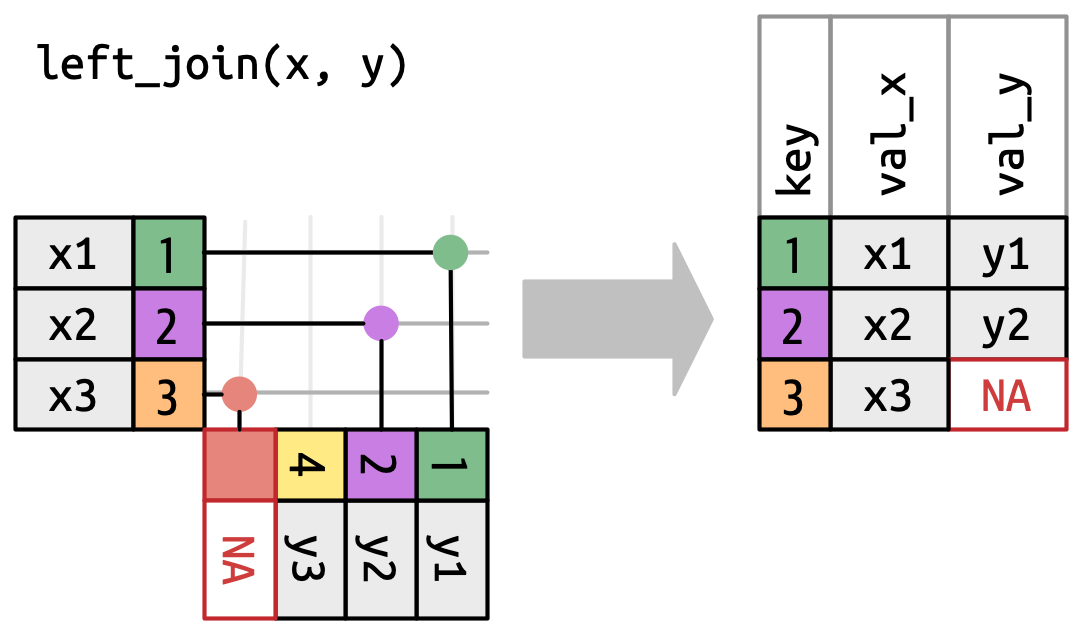
\includegraphics[width=4.41667in,height=\textheight]{images/clipboard-1594422253.png}

}

\caption{A visual representation of the left join where every row in x
appears in the output.Source: R for Data Science.}

\end{figure}%

Let's \textbf{join the municipalities} to this table with a supporting
table that includes all the \textbf{relation} between neighbourhoods and
municipalities, and the respective names and codes.

\begin{Shaded}
\begin{Highlighting}[]
\NormalTok{Municipalities }\OtherTok{=} \FunctionTok{readRDS}\NormalTok{(}\StringTok{"data/Municipalities\_names.Rds"}\NormalTok{)}
\end{Highlighting}
\end{Shaded}

\begin{Shaded}
\begin{Highlighting}[]
\FunctionTok{head}\NormalTok{(TRIPS)}
\end{Highlighting}
\end{Shaded}

\begin{verbatim}
# A tibble: 6 x 13
  Origin Total  Walk  Bike   Car PTransit Other Internal Lisbon Car_perc
  <chr>  <dbl> <dbl> <dbl> <dbl>    <dbl> <dbl>    <dbl>  <dbl>    <dbl>
1 110501 35539 11325  1309 21446     1460     0        0      0     60.3
2 110501 47602  3502   416 37727     5519   437        1      0     79.3
3 110506 37183 12645    40 22379     2057    63        0      0     60.2
4 110506 42313  1418   163 37337     3285   106        1      0     88.2
5 110507 30725  9389  1481 19654      201     0        0      0     64.0
6 110507 54586  2630   168 44611     6963   215        1      0     81.7
# i 3 more variables: Origin_num <int>, Lisbon_factor <fct>,
#   Internal_factor <fct>
\end{verbatim}

\begin{Shaded}
\begin{Highlighting}[]
\FunctionTok{tail}\NormalTok{(Municipalities)}
\end{Highlighting}
\end{Shaded}

\begin{verbatim}
    Mun_code Neighborhood_code        Municipality
113     1109            110913               Mafra
114     1114            111409 Vila Franca de Xira
115     1109            110918               Mafra
116     1109            110904               Mafra
117     1502            150202           Alcochete
118     1109            110911               Mafra
                                             Neighborhood
113                                         Santo Isidoro
114                                   Vila Franca de Xira
115 União das freguesias de Azueira e Sobral da Abelheira
116                                            Encarnação
117                                               Samouco
118                                             Milharado
\end{verbatim}

We can see that we have a common variable: \texttt{Origin} in
\texttt{TRIPS} and \texttt{Neighborhood\_code} in
\texttt{Municipalities}.

To join these two tables we need to specify the common variable in each
table, using the \texttt{by} argument.

\begin{Shaded}
\begin{Highlighting}[]
\NormalTok{TRIPSjoin }\OtherTok{=}\NormalTok{ TRIPS }\SpecialCharTok{|\textgreater{}} \FunctionTok{left\_join}\NormalTok{(Municipalities, }\AttributeTok{by =} \FunctionTok{c}\NormalTok{(}\StringTok{"Origin"} \OtherTok{=} \StringTok{"Neighborhood\_code"}\NormalTok{))}
\end{Highlighting}
\end{Shaded}

If you prefer, you can mutate or rename a variable so both tables have
the same name. When \textbf{both tables have the same name}, you don't
need to specify the \texttt{by} argument.

\begin{Shaded}
\begin{Highlighting}[]
\NormalTok{Municipalities }\OtherTok{=}\NormalTok{ Municipalities }\SpecialCharTok{|\textgreater{}} \FunctionTok{rename}\NormalTok{(}\AttributeTok{Origin =} \StringTok{"Neighborhood\_code"}\NormalTok{) }\CommentTok{\# change name}
\NormalTok{TRIPSjoin }\OtherTok{=}\NormalTok{ TRIPS }\SpecialCharTok{|\textgreater{}} \FunctionTok{left\_join}\NormalTok{(Municipalities) }\CommentTok{\# automatic detects common variable}
\end{Highlighting}
\end{Shaded}

As you can see, both tables don't need to be the same length. The
\texttt{left\_join} function will keep all the observations from the
first table, and join the second table to it. If there is no match, the
variables from the second table will be filled with \texttt{NA}.

\section{group\_by and summarize}\label{group_by-and-summarize}

We have a very large table with all the neighbourhoods and their
respective municipalities. We want to know the total number of trips
with origin in each municipality.

To make it easier to understand, let's keep only the variables we need.

\begin{Shaded}
\begin{Highlighting}[]
\NormalTok{TRIPSredux }\OtherTok{=}\NormalTok{ TRIPSjoin }\SpecialCharTok{|\textgreater{}} \FunctionTok{select}\NormalTok{(Origin, Municipality, Internal, Car, Total)}
\FunctionTok{head}\NormalTok{(TRIPSredux)}
\end{Highlighting}
\end{Shaded}

\begin{verbatim}
# A tibble: 6 x 5
  Origin Municipality Internal   Car Total
  <chr>  <chr>           <dbl> <dbl> <dbl>
1 110501 Cascais             0 21446 35539
2 110501 Cascais             1 37727 47602
3 110506 Cascais             0 22379 37183
4 110506 Cascais             1 37337 42313
5 110507 Cascais             0 19654 30725
6 110507 Cascais             1 44611 54586
\end{verbatim}

We can group this table by the \texttt{Municipality} variable and
summarize the number of trips with origin in each municipality.

\begin{Shaded}
\begin{Highlighting}[]
\NormalTok{TRIPSsum }\OtherTok{=}\NormalTok{ TRIPSredux }\SpecialCharTok{|\textgreater{}} 
  \FunctionTok{group\_by}\NormalTok{(Municipality) }\SpecialCharTok{|\textgreater{}} \CommentTok{\# you won\textquotesingle{}t notice any chagne with only this}
  \FunctionTok{summarize}\NormalTok{(}\AttributeTok{Total =} \FunctionTok{sum}\NormalTok{(Total))}
\FunctionTok{head}\NormalTok{(TRIPSsum)}
\end{Highlighting}
\end{Shaded}

\begin{verbatim}
# A tibble: 6 x 2
  Municipality   Total
  <chr>          <dbl>
1 Alcochete      36789
2 Almada        289834
3 Amadora       344552
4 Barreiro      133658
5 Cascais       373579
6 Lisboa       1365111
\end{verbatim}

We summed the total number of trips in each municipality.

If we want to group by more than one variable, we can add more
\texttt{group\_by()} functions.

\begin{Shaded}
\begin{Highlighting}[]
\NormalTok{TRIPSsum2 }\OtherTok{=}\NormalTok{ TRIPSredux }\SpecialCharTok{|\textgreater{}} 
  \FunctionTok{group\_by}\NormalTok{(Municipality, Internal) }\SpecialCharTok{|\textgreater{}} 
  \FunctionTok{summarize}\NormalTok{(}\AttributeTok{Total =} \FunctionTok{sum}\NormalTok{(Total),}
            \AttributeTok{Car =} \FunctionTok{sum}\NormalTok{(Car))}
\FunctionTok{head}\NormalTok{(TRIPSsum2)}
\end{Highlighting}
\end{Shaded}

\begin{verbatim}
# A tibble: 6 x 4
# Groups:   Municipality [3]
  Municipality Internal  Total    Car
  <chr>           <dbl>  <dbl>  <dbl>
1 Alcochete           0  16954   9839
2 Alcochete           1  19835  15632
3 Almada              0 105841  49012
4 Almada              1 183993 125091
5 Amadora             0 117727  33818
6 Amadora             1 226825 142386
\end{verbatim}

We summed the total number of trips and car trips in each municipality,
\textbf{separated by} inter and intra municipal trips.

\begin{tcolorbox}[enhanced jigsaw, breakable, left=2mm, colframe=quarto-callout-caution-color-frame, leftrule=.75mm, bottomrule=.15mm, arc=.35mm, rightrule=.15mm, colback=white, opacityback=0, toprule=.15mm]
\begin{minipage}[t]{5.5mm}
\textcolor{quarto-callout-caution-color}{\faFire}
\end{minipage}%
\begin{minipage}[t]{\textwidth - 5.5mm}

It is a good practice to use the \texttt{ungroup()} function after the
\texttt{group\_by()} function. This will remove the grouping. If you
don't do this, the grouping will be kept and you may have unexpected
results in the next time you use that dataset.

\end{minipage}%
\end{tcolorbox}

\section{Arrange data}\label{arrange-data}

You can \textbf{sort} a dataset by one or more variables.

For instance, \texttt{arrange()} by Total trips, ascending or descending
order.

\begin{Shaded}
\begin{Highlighting}[]
\NormalTok{TRIPS2 }\OtherTok{=}\NormalTok{ TRIPSsum2 }\SpecialCharTok{|\textgreater{}} \FunctionTok{arrange}\NormalTok{(Total)}
\NormalTok{TRIPS2 }\OtherTok{=}\NormalTok{ TRIPSsum2 }\SpecialCharTok{|\textgreater{}} \FunctionTok{arrange}\NormalTok{(}\SpecialCharTok{{-}}\NormalTok{Total) }\CommentTok{\# descending}

\NormalTok{TRIPS2 }\OtherTok{=}\NormalTok{ TRIPSsum2 }\SpecialCharTok{|\textgreater{}} \FunctionTok{arrange}\NormalTok{(Municipality) }\CommentTok{\# alphabetic}

\NormalTok{TRIPS4 }\OtherTok{=}\NormalTok{ TRIPS }\SpecialCharTok{|\textgreater{}} \FunctionTok{arrange}\NormalTok{(Lisbon\_factor, Total) }\CommentTok{\# more than one variable}
\end{Highlighting}
\end{Shaded}

This is not the same as opening the view table and click on the arrows.
When you do that, the order is not saved in the dataset. If you want to
save the order, you need to use the \texttt{arrange()} function.

\section{All together now!}\label{all-together-now}

This is the pipes magic. It takes the last result and applies the next
function to it. ``With this, do this.''. You can chain as many functions
as you want.

\begin{Shaded}
\begin{Highlighting}[]
\NormalTok{TRIPS\_pipes }\OtherTok{=}\NormalTok{ TRIPS }\SpecialCharTok{|\textgreater{}} 
  \FunctionTok{select}\NormalTok{(Origin, Internal, Car, Total) }\SpecialCharTok{|\textgreater{}} 
  
  \FunctionTok{mutate}\NormalTok{(}\AttributeTok{Origin\_num =} \FunctionTok{as.integer}\NormalTok{(Origin)) }\SpecialCharTok{|\textgreater{}} 
  \FunctionTok{mutate}\NormalTok{(}\AttributeTok{Internal\_factor =} \FunctionTok{factor}\NormalTok{(Internal, }\AttributeTok{labels =} \FunctionTok{c}\NormalTok{(}\StringTok{"Inter"}\NormalTok{, }\StringTok{"Intra"}\NormalTok{))) }\SpecialCharTok{|\textgreater{}} 
  
  \FunctionTok{filter}\NormalTok{(Internal\_factor }\SpecialCharTok{==} \StringTok{"Inter"}\NormalTok{)}\SpecialCharTok{|\textgreater{}}
  
  \FunctionTok{left\_join}\NormalTok{(Municipalities) }\SpecialCharTok{|\textgreater{}}
  
  \FunctionTok{group\_by}\NormalTok{(Municipality) }\SpecialCharTok{|\textgreater{}}
  \FunctionTok{summarize}\NormalTok{(}\AttributeTok{Total =} \FunctionTok{sum}\NormalTok{(Total),}
            \AttributeTok{Car =} \FunctionTok{sum}\NormalTok{(Car),}
            \AttributeTok{Car\_perc =}\NormalTok{ Car}\SpecialCharTok{/}\NormalTok{Total }\SpecialCharTok{*} \DecValTok{100}\NormalTok{) }\SpecialCharTok{|\textgreater{}} 
  \FunctionTok{ungroup}\NormalTok{() }\SpecialCharTok{|\textgreater{}} 
  
  \FunctionTok{arrange}\NormalTok{(}\FunctionTok{desc}\NormalTok{(Car\_perc))}
\end{Highlighting}
\end{Shaded}

With this code we will have a table with the total number of intercity
trips, by municipality, with their names instead of codes, arranged by
the percentage of car trips.

\begin{Shaded}
\begin{Highlighting}[]
\NormalTok{TRIPS\_pipes}
\end{Highlighting}
\end{Shaded}

\begin{verbatim}
# A tibble: 18 x 4
   Municipality         Total    Car Car_perc
   <chr>                <dbl>  <dbl>    <dbl>
 1 Mafra                65811  46329     70.4
 2 Sesimbra             49370  31975     64.8
 3 Cascais             161194  96523     59.9
 4 Palmela              66428  39688     59.7
 5 Alcochete            16954   9839     58.0
 6 Setúbal             129059  70318     54.5
 7 Montijo              57164  30900     54.1
 8 Seixal              120747  63070     52.2
 9 Sintra              237445 123408     52.0
10 Oeiras              134862  66972     49.7
11 Almada              105841  49012     46.3
12 Loures              132310  60478     45.7
13 Barreiro             52962  24160     45.6
14 Odivelas             93709  39151     41.8
15 Vila Franca de Xira 115152  47201     41.0
16 Moita                51040  17394     34.1
17 Amadora             117727  33818     28.7
18 Lisboa              280079  69038     24.6
\end{verbatim}

\section{Other dplyr functions}\label{other-dplyr-functions}

You can explore other \texttt{dplyr} functions and variations to
manipulate data in the \textbf{dplyr cheat sheet}:

\href{https://rstudio.github.io/cheatsheets/data-transformation.pdf}{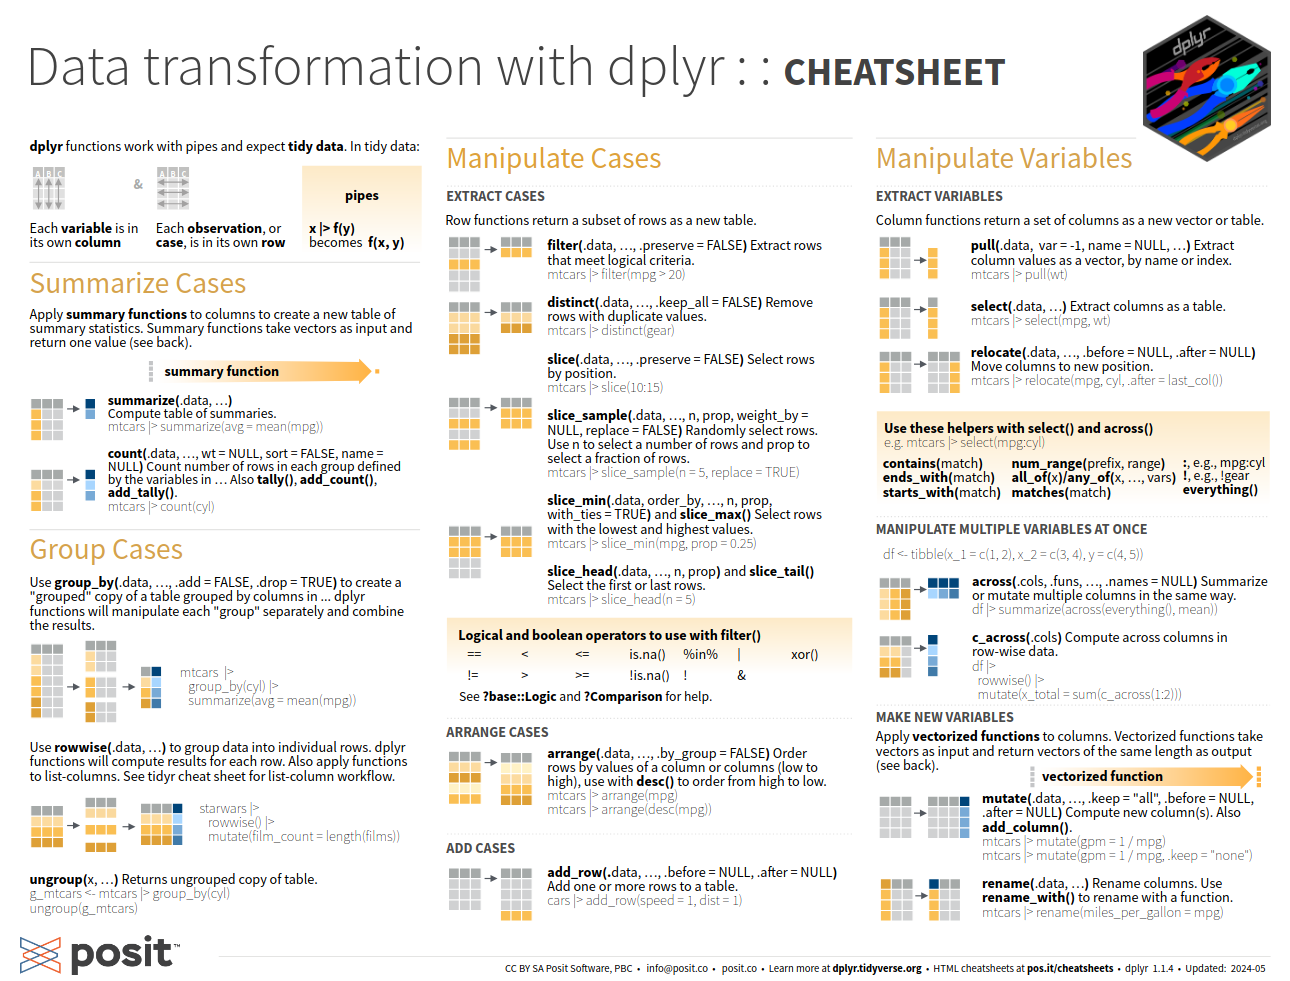
\includegraphics{images/clipboard-2101323289.png}}

Take a particular attention to \texttt{pivot\_wider} and
\texttt{pivot\_longer}
(\href{https://tidyr.tidyverse.org/articles/pivot.html}{\texttt{tidyr}}
package) to transform \textbf{OD matrices} in \textbf{wide} and
\textbf{long} formats.

\begin{longtable}[]{@{}llr@{}}
\caption{OD matrix in long format}\tabularnewline
\toprule\noalign{}
Origins & Destinations & Trips \\
\midrule\noalign{}
\endfirsthead
\toprule\noalign{}
Origins & Destinations & Trips \\
\midrule\noalign{}
\endhead
\bottomrule\noalign{}
\endlastfoot
A & B & 20 \\
A & C & 45 \\
B & A & 10 \\
C & C & 5 \\
C & A & 30 \\
\end{longtable}

\begin{longtable}[]{@{}lrrr@{}}
\caption{OD matrix in wide format}\tabularnewline
\toprule\noalign{}
Trips & A & B & C \\
\midrule\noalign{}
\endfirsthead
\toprule\noalign{}
Trips & A & B & C \\
\midrule\noalign{}
\endhead
\bottomrule\noalign{}
\endlastfoot
A & NA & 20 & 45 \\
B & 10 & NA & NA \\
C & 30 & NA & 5 \\
\end{longtable}

\chapter{Introduction to spatial
data}\label{introduction-to-spatial-data}

Spatial data is \textbf{data that is associated with a geometry}. This
geometry can be a point, a line, a polygon, or a grid.

Spatial data can be represented in many ways, such as vector data and
raster data. In this tutorial, we will learn how to work with spatial
data in R.

We will use the \texttt{sf} package to work with vector data, and the
\texttt{dplyr} package to manipulate data.

\begin{Shaded}
\begin{Highlighting}[]
\FunctionTok{library}\NormalTok{(sf)}
\FunctionTok{library}\NormalTok{(dplyr)}
\end{Highlighting}
\end{Shaded}

The \texttt{sf} package is a powerful package for working with spatial
data in R. It includes hundreds of
\href{https://r-spatial.github.io/sf/reference/index.html}{functions} to
deal with spatial data (Pebesma and Bivand 2023).

\section{Import vector data}\label{import-vector-data}

Download and open \texttt{Municipalities\_geo.gpkg} under
\href{https://github.com/U-Shift/EITcourse/tree/main/data}{EITcourse/data}
repository.

Within the \texttt{sf} package, we use the \texttt{st\_read()} to read
spatial features.

\begin{Shaded}
\begin{Highlighting}[]
\NormalTok{Municipalities\_geo }\OtherTok{=} \FunctionTok{st\_read}\NormalTok{(}\StringTok{"data/Municipalities\_geo.gpkg"}\NormalTok{)}
\end{Highlighting}
\end{Shaded}

\begin{verbatim}
Reading layer `Municipalities_geo' from data source 
  `D:\GIS\EITcourse\data\Municipalities_geo.gpkg' using driver `GPKG'
Simple feature collection with 18 features and 1 field
Geometry type: MULTIPOLYGON
Dimension:     XY
Bounding box:  xmin: -9.500527 ymin: 38.40907 xmax: -8.490972 ymax: 39.06472
Geodetic CRS:  WGS 84
\end{verbatim}

\begin{tcolorbox}[enhanced jigsaw, breakable, left=2mm, colframe=quarto-callout-tip-color-frame, leftrule=.75mm, bottomrule=.15mm, arc=.35mm, rightrule=.15mm, colback=white, opacityback=0, toprule=.15mm]
\begin{minipage}[t]{5.5mm}
\textcolor{quarto-callout-tip-color}{\faLightbulb}
\end{minipage}%
\begin{minipage}[t]{\textwidth - 5.5mm}

You can also open directly from url from github. Example:

\texttt{Municipalities\_geo\ =\ st\_read("https://github.com/U-Shift/EITcourse/raw/main/data/Municipalities\_geo.gpkg")}

\end{minipage}%
\end{tcolorbox}

\subsection{Projected vs Geographic Coordinate
Systems}\label{projected-vs-geographic-coordinate-systems}

A \textbf{projected coordinate system} is a flat representation of the
Earth's surface. A \textbf{geographic coordinate system} is a spherical
representation of the Earth's surface.

\begin{figure}[H]

{\centering 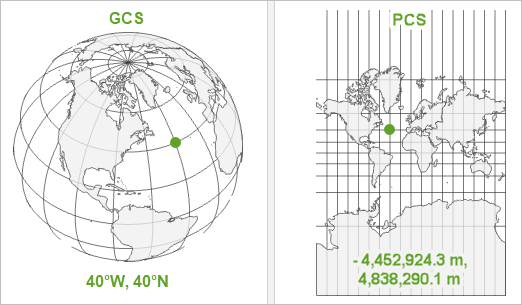
\includegraphics{images/clipboard-1233124217.png}

}

\caption{Source: ESRI}

\end{figure}%

The \texttt{st\_crs()} function can be used to check the
\textbf{coordinate reference system} of a spatial object.

\begin{Shaded}
\begin{Highlighting}[]
\FunctionTok{st\_crs}\NormalTok{(Municipalities\_geo)}
\end{Highlighting}
\end{Shaded}

\begin{verbatim}
Coordinate Reference System:
  User input: WGS 84 
  wkt:
GEOGCRS["WGS 84",
    ENSEMBLE["World Geodetic System 1984 ensemble",
        MEMBER["World Geodetic System 1984 (Transit)"],
        MEMBER["World Geodetic System 1984 (G730)"],
        MEMBER["World Geodetic System 1984 (G873)"],
        MEMBER["World Geodetic System 1984 (G1150)"],
        MEMBER["World Geodetic System 1984 (G1674)"],
        MEMBER["World Geodetic System 1984 (G1762)"],
        MEMBER["World Geodetic System 1984 (G2139)"],
        ELLIPSOID["WGS 84",6378137,298.257223563,
            LENGTHUNIT["metre",1]],
        ENSEMBLEACCURACY[2.0]],
    PRIMEM["Greenwich",0,
        ANGLEUNIT["degree",0.0174532925199433]],
    CS[ellipsoidal,2],
        AXIS["geodetic latitude (Lat)",north,
            ORDER[1],
            ANGLEUNIT["degree",0.0174532925199433]],
        AXIS["geodetic longitude (Lon)",east,
            ORDER[2],
            ANGLEUNIT["degree",0.0174532925199433]],
    USAGE[
        SCOPE["Horizontal component of 3D system."],
        AREA["World."],
        BBOX[-90,-180,90,180]],
    ID["EPSG",4326]]
\end{verbatim}

WGS84 is the most common geographic coordinate system, used in GPS, and
\href{https://epsg.io/4326}{EPSG:\textbf{4326}} is code for it.

If we want to project the data to a projected coordinate system, to use
\textbf{metric units} instead of degrees, we can use the
\texttt{st\_transform()} function.

In this case, the \href{https://epsg.io/3857}{EPGS:\textbf{3857}} is the
code for the Pseudo-Mercator coordinate system.

\begin{Shaded}
\begin{Highlighting}[]
\NormalTok{Municipalities\_projected }\OtherTok{=} \FunctionTok{st\_transform}\NormalTok{(Municipalities\_geo, }\AttributeTok{crs =} \DecValTok{3857}\NormalTok{)}
\end{Highlighting}
\end{Shaded}

Now see the differences when calling \texttt{Municipalities\_geo} and
\texttt{Municipalities\_projected.}

\section{Join geometries to data
frames}\label{join-geometries-to-data-frames}

Import \texttt{TRIPSmun.Rds} file and check data class-

\begin{Shaded}
\begin{Highlighting}[]
\NormalTok{TRIPSmun }\OtherTok{=} \FunctionTok{readRDS}\NormalTok{(}\StringTok{"data/TRIPSmun.Rds"}\NormalTok{)}
\FunctionTok{class}\NormalTok{(TRIPSmun)}
\end{Highlighting}
\end{Shaded}

\begin{verbatim}
[1] "data.frame"
\end{verbatim}

\begin{Shaded}
\begin{Highlighting}[]
\FunctionTok{class}\NormalTok{(Municipalities\_geo)}
\end{Highlighting}
\end{Shaded}

\begin{verbatim}
[1] "sf"         "data.frame"
\end{verbatim}

To join the geometries from the \texttt{Municipalities\_geo} to the data
frame, we can use the \texttt{left\_join()} function from the
\texttt{dplyr} package.

\begin{Shaded}
\begin{Highlighting}[]
\NormalTok{TRIPSgeo }\OtherTok{=}
\NormalTok{  TRIPSmun }\SpecialCharTok{|\textgreater{}} 
  \FunctionTok{left\_join}\NormalTok{(Municipalities\_geo)}

\FunctionTok{class}\NormalTok{(TRIPSgeo)}
\end{Highlighting}
\end{Shaded}

\begin{verbatim}
[1] "data.frame"
\end{verbatim}

As you can see, this \textbf{does not make the object a spatial
feature}. To do this, we need to use the \texttt{st\_as\_sf()} function.

\begin{Shaded}
\begin{Highlighting}[]
\NormalTok{TRIPSgeo }\OtherTok{=}\NormalTok{ TRIPSgeo }\SpecialCharTok{|\textgreater{}} \FunctionTok{st\_as\_sf}\NormalTok{()}
\FunctionTok{class}\NormalTok{(TRIPSgeo)}
\end{Highlighting}
\end{Shaded}

\begin{verbatim}
[1] "sf"         "data.frame"
\end{verbatim}

Now we have a spatial feature with the data frame.

\section{Create spatial data from
coordinates}\label{create-spatial-data-from-coordinates}

The \texttt{st\_as\_sf()} function can also be used to create a spatial
feature from a data frame with coordinates. In that case, we need to
specify the columns with the coordinates.

We will use survey data (in \texttt{.txt}) with the participants' home
latitude/longitude coordinates to create a spatial feature.

\begin{Shaded}
\begin{Highlighting}[]
\NormalTok{SURVEY }\OtherTok{=} \FunctionTok{read.csv}\NormalTok{(}\StringTok{"data/SURVEY.txt"}\NormalTok{, }\AttributeTok{sep =} \StringTok{"}\SpecialCharTok{\textbackslash{}t}\StringTok{"}\NormalTok{) }\CommentTok{\# tab delimiter}
\FunctionTok{class}\NormalTok{(SURVEY)}
\end{Highlighting}
\end{Shaded}

\begin{verbatim}
[1] "data.frame"
\end{verbatim}

\begin{Shaded}
\begin{Highlighting}[]
\NormalTok{SURVEYgeo }\OtherTok{=} \FunctionTok{st\_as\_sf}\NormalTok{(SURVEY, }\AttributeTok{coords =} \FunctionTok{c}\NormalTok{(}\StringTok{"lon"}\NormalTok{, }\StringTok{"lat"}\NormalTok{), }\AttributeTok{crs =} \DecValTok{4326}\NormalTok{) }\CommentTok{\# create spatial feature}
\FunctionTok{class}\NormalTok{(SURVEYgeo)}
\end{Highlighting}
\end{Shaded}

\begin{verbatim}
[1] "sf"         "data.frame"
\end{verbatim}

We can also set the \textbf{crs} of the spatial feature on the fly.

Check the differences between both data variables.

\section{Visuzlize spatial data}\label{visuzlize-spatial-data}

Represent Transport Zones with Total and Car, using \texttt{plot()}.

\begin{Shaded}
\begin{Highlighting}[]
\FunctionTok{plot}\NormalTok{(TRIPSgeo) }\CommentTok{\# all variables}
\end{Highlighting}
\end{Shaded}

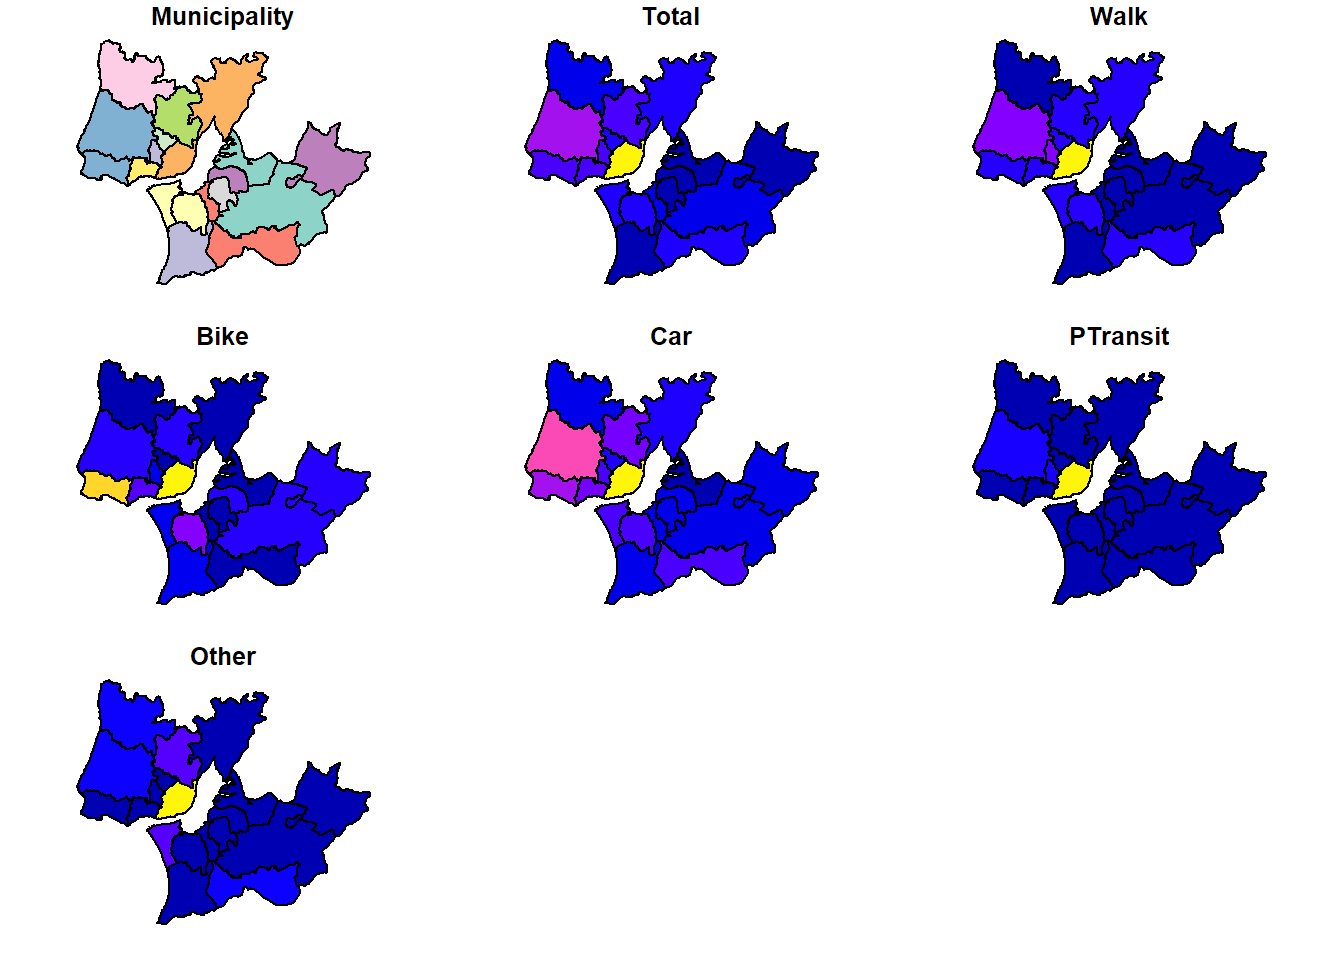
\includegraphics{spatial-data_files/figure-pdf/unnamed-chunk-10-1.pdf}

\begin{Shaded}
\begin{Highlighting}[]
\FunctionTok{plot}\NormalTok{(TRIPSgeo[}\StringTok{"Municipality"}\NormalTok{])}
\end{Highlighting}
\end{Shaded}

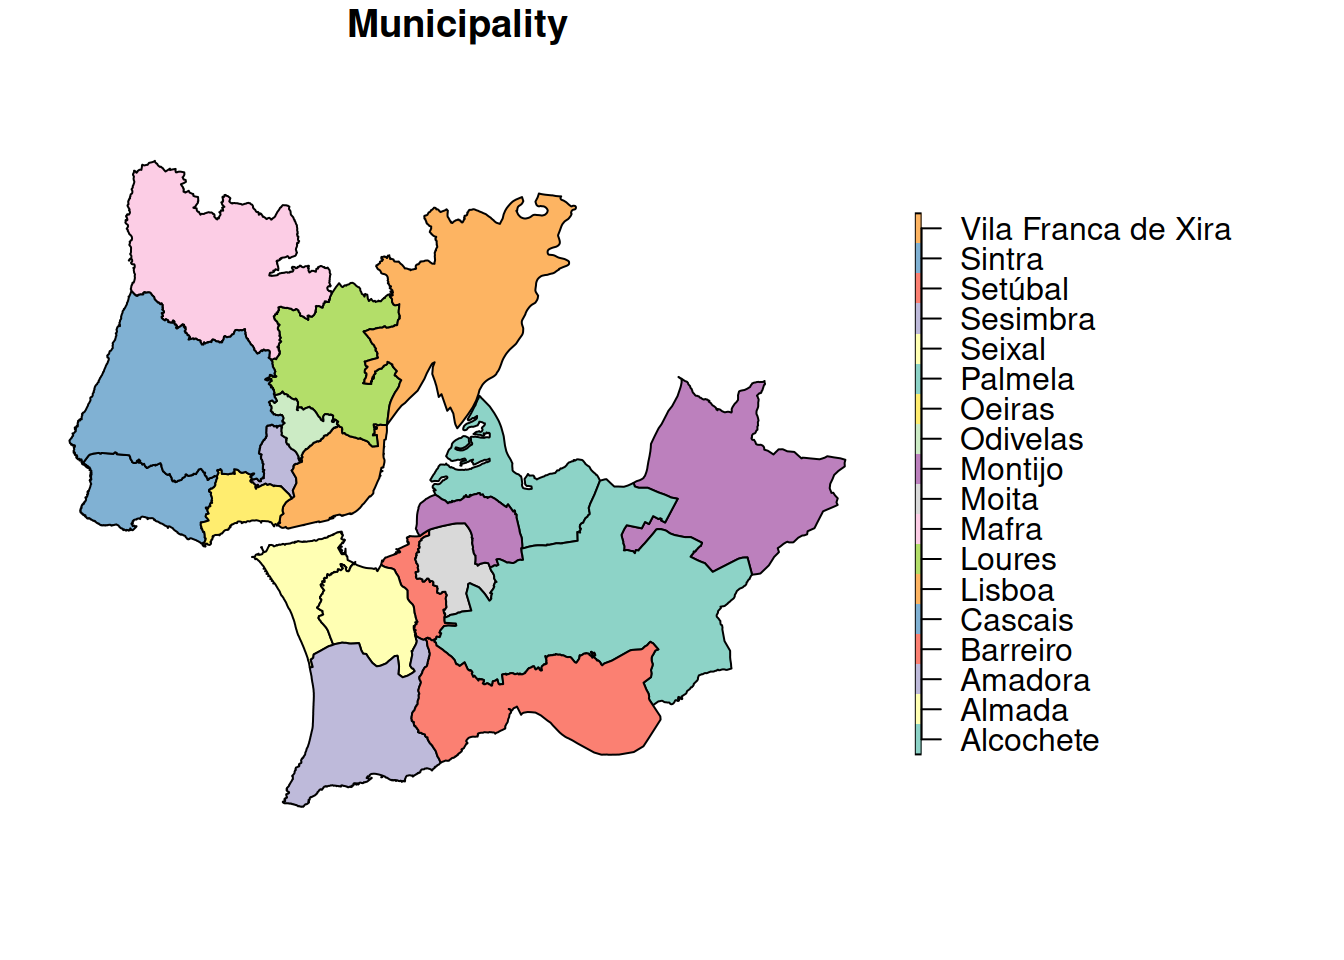
\includegraphics{spatial-data_files/figure-pdf/unnamed-chunk-10-2.pdf}

\begin{Shaded}
\begin{Highlighting}[]
\FunctionTok{plot}\NormalTok{(TRIPSgeo[}\StringTok{"Total"}\NormalTok{])}
\end{Highlighting}
\end{Shaded}

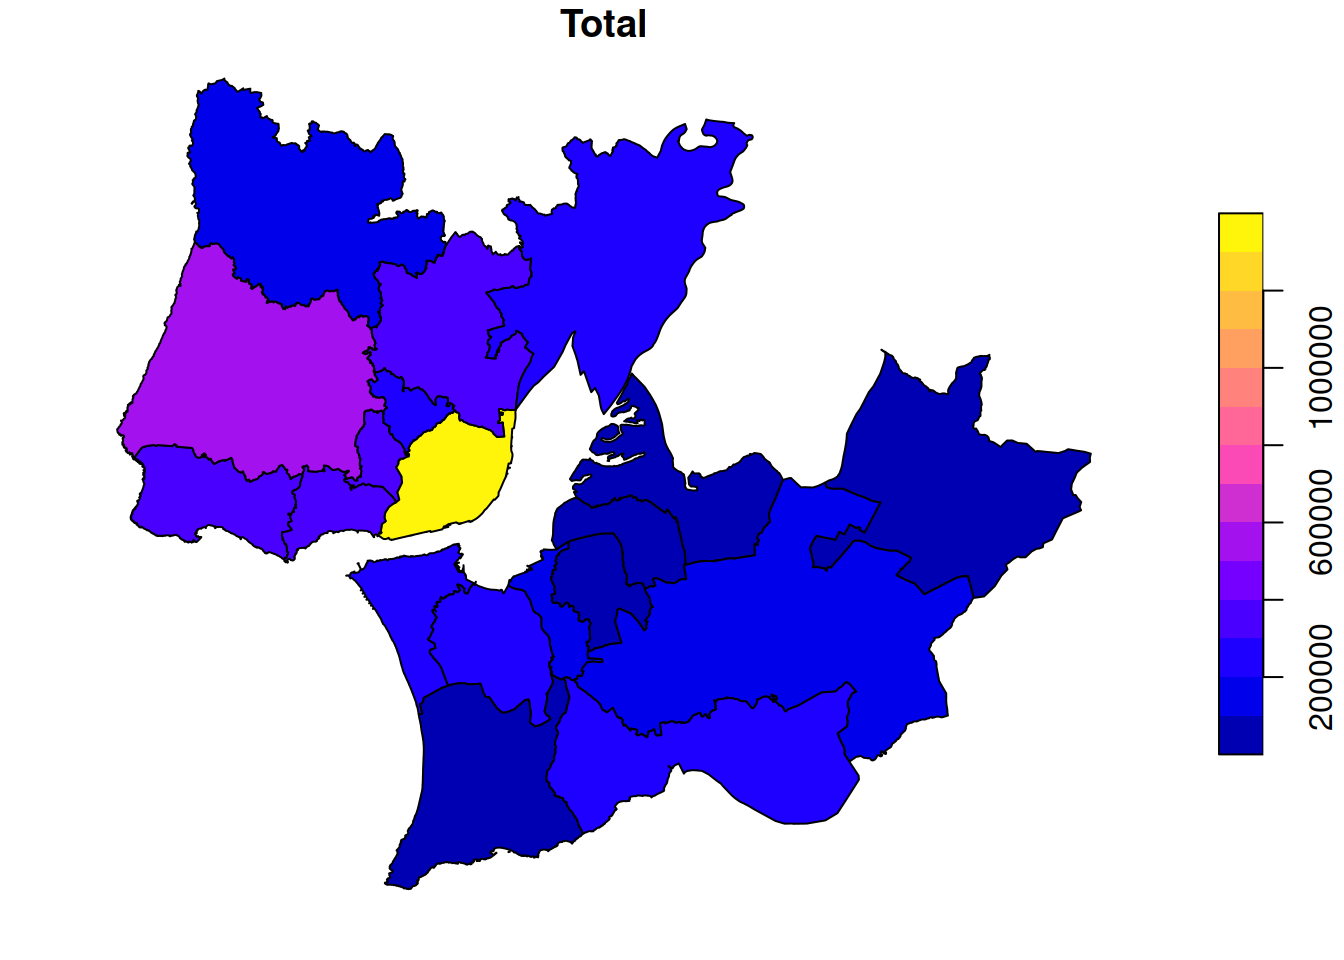
\includegraphics{spatial-data_files/figure-pdf/unnamed-chunk-10-3.pdf}

\begin{Shaded}
\begin{Highlighting}[]
\FunctionTok{plot}\NormalTok{(TRIPSgeo[}\StringTok{"Car"}\NormalTok{])}
\end{Highlighting}
\end{Shaded}

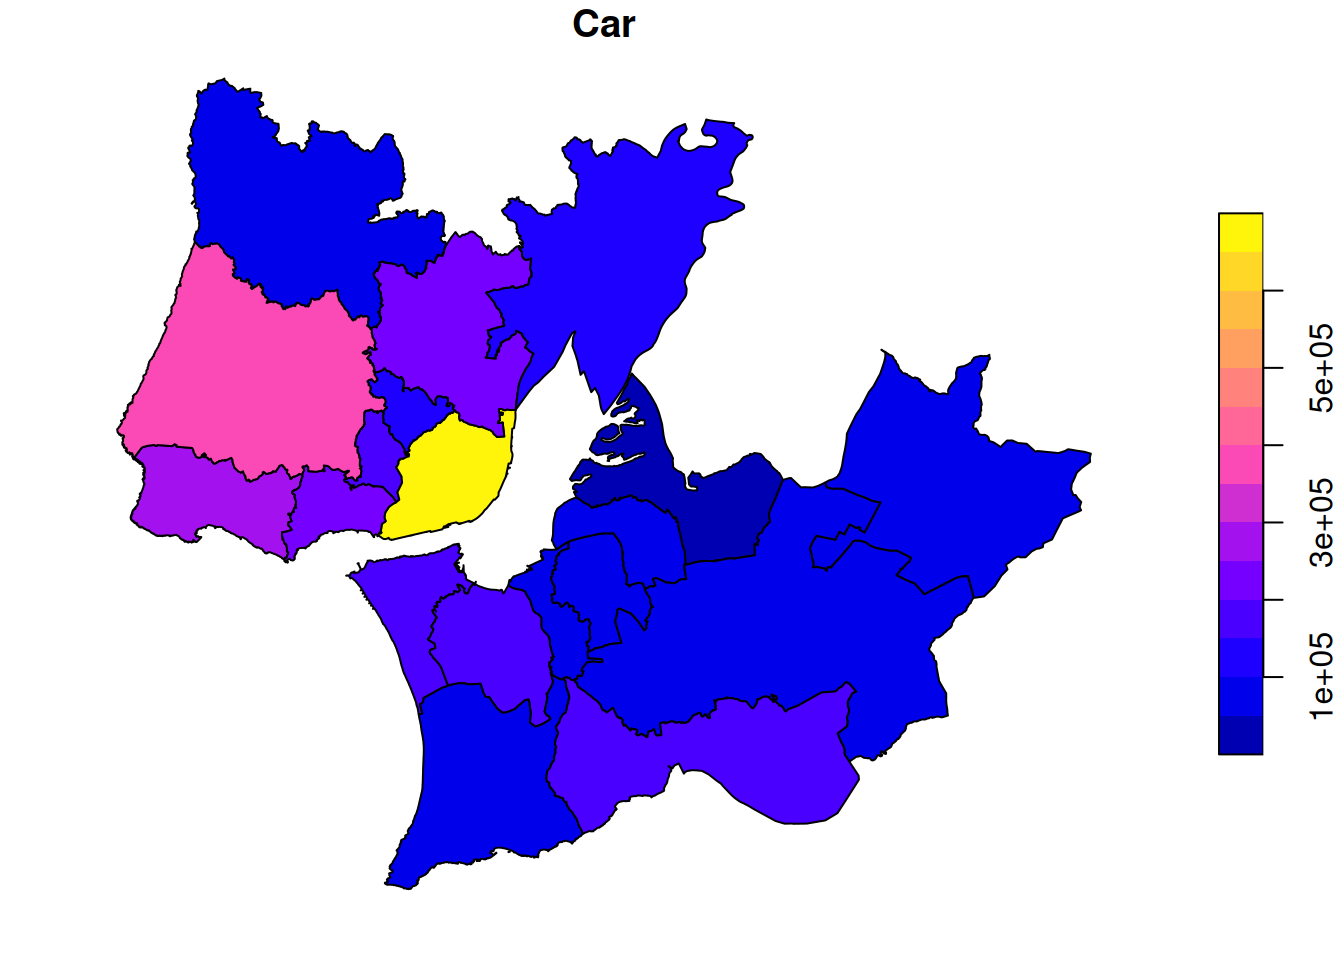
\includegraphics{spatial-data_files/figure-pdf/unnamed-chunk-10-4.pdf}

\begin{Shaded}
\begin{Highlighting}[]
\CommentTok{\# plot pointy data}
\FunctionTok{plot}\NormalTok{(SURVEYgeo)}
\end{Highlighting}
\end{Shaded}

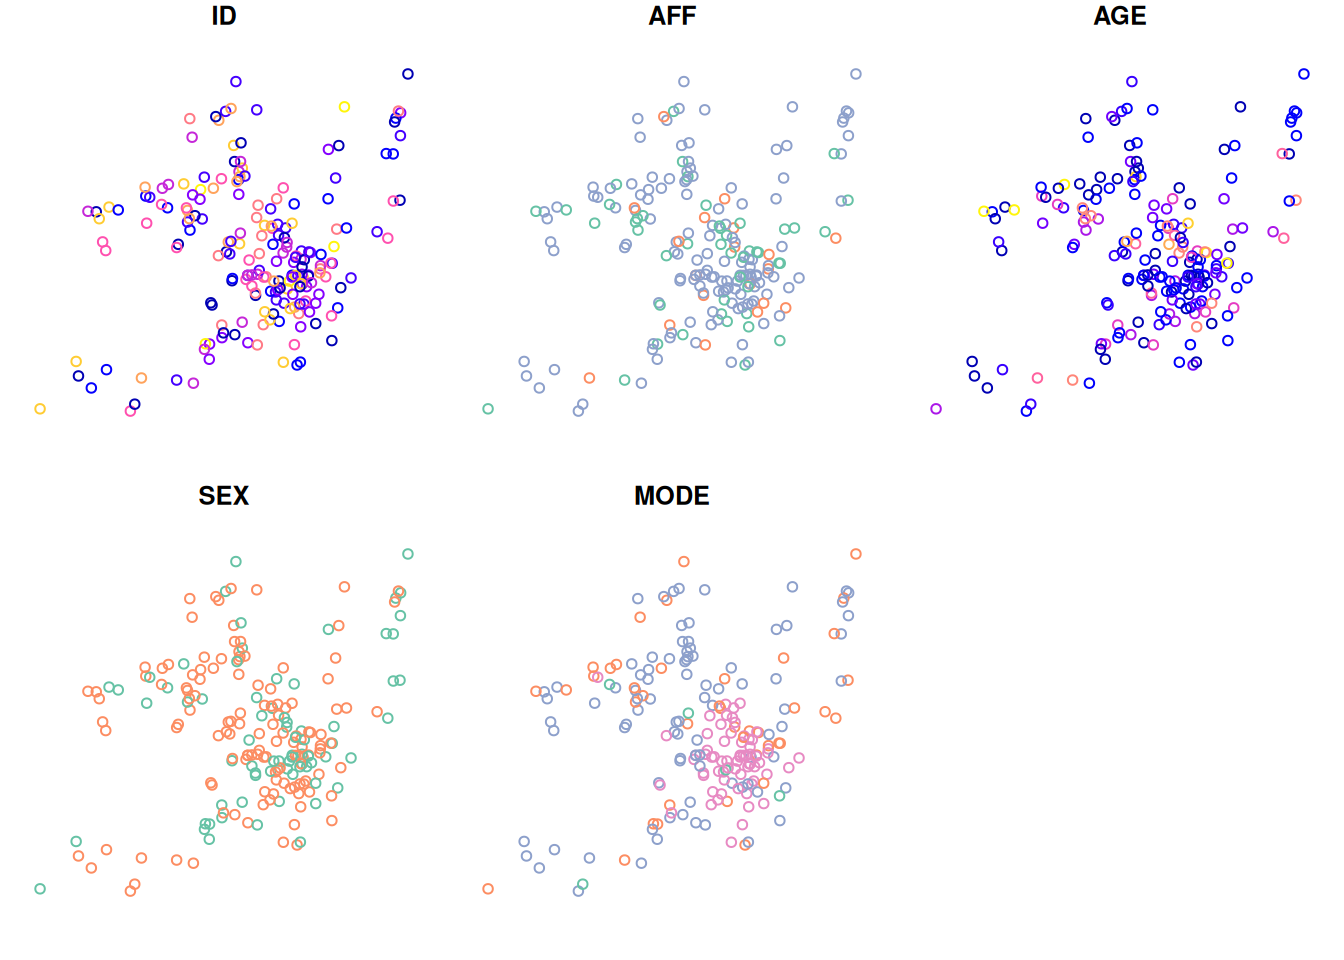
\includegraphics{spatial-data_files/figure-pdf/unnamed-chunk-10-5.pdf}

\begin{tcolorbox}[enhanced jigsaw, breakable, left=2mm, colframe=quarto-callout-note-color-frame, leftrule=.75mm, bottomrule=.15mm, arc=.35mm, rightrule=.15mm, colback=white, opacityback=0, toprule=.15mm]
\begin{minipage}[t]{5.5mm}
\textcolor{quarto-callout-note-color}{\faInfo}
\end{minipage}%
\begin{minipage}[t]{\textwidth - 5.5mm}

In the next chapter we will learn how to create interactive maps.

\end{minipage}%
\end{tcolorbox}

\section{Export spatial data}\label{export-spatial-data}

You can save your spatial data in different formats using the function
\texttt{st\_write()}, such as shapefiles (ESRI), GeoJSON, and
GeoPackage.

This is also useful to convert spatial data between formats.

\begin{Shaded}
\begin{Highlighting}[]
\FunctionTok{st\_write}\NormalTok{(TRIPSgeo, }\StringTok{"data/TRIPSgeo.gpkg"}\NormalTok{) }\CommentTok{\# as geopackage}
\FunctionTok{st\_write}\NormalTok{(TRIPSgeo, }\StringTok{"data/TRIPSgeo.shp"}\NormalTok{) }\CommentTok{\# as shapefile}
\FunctionTok{st\_write}\NormalTok{(TRIPSgeo, }\StringTok{"data/TRIPSgeo.geojson"}\NormalTok{) }\CommentTok{\# as geojson}
\FunctionTok{st\_write}\NormalTok{(TRIPSgeo, }\StringTok{"data/TRIPSgeo.csv"}\NormalTok{, }\AttributeTok{layer\_options =} \StringTok{"GEOMETRY=AS\_WKT"}\NormalTok{) }\CommentTok{\# as csv, with WKT geometry}
\end{Highlighting}
\end{Shaded}

\begin{tcolorbox}[enhanced jigsaw, breakable, left=2mm, colframe=quarto-callout-warning-color-frame, leftrule=.75mm, bottomrule=.15mm, arc=.35mm, rightrule=.15mm, colback=white, opacityback=0, toprule=.15mm]
\begin{minipage}[t]{5.5mm}
\textcolor{quarto-callout-warning-color}{\faExclamationTriangle}
\end{minipage}%
\begin{minipage}[t]{\textwidth - 5.5mm}

If you already have a file with the same name, you can use the
\texttt{delete\_dns\ =\ TRUE} argument to overwrite it.

\end{minipage}%
\end{tcolorbox}

\chapter{Interactive maps}\label{interactive-maps}

You can plot a static map using \texttt{plof(sf)}, but you can also
create interactive maps.

\begin{Shaded}
\begin{Highlighting}[]
\FunctionTok{library}\NormalTok{(sf)}
\NormalTok{TRIPSgeo }\OtherTok{=} \FunctionTok{st\_read}\NormalTok{(}\StringTok{"data/TRIPSgeo.gpkg"}\NormalTok{)}
\end{Highlighting}
\end{Shaded}

\begin{verbatim}
Reading layer `TRIPSgeo' from data source `D:\GIS\EITcourse\data\TRIPSgeo.gpkg' using driver `GPKG'
Simple feature collection with 18 features and 7 fields
Geometry type: MULTIPOLYGON
Dimension:     XY
Bounding box:  xmin: -9.500527 ymin: 38.40907 xmax: -8.490972 ymax: 39.06472
Geodetic CRS:  WGS 84
\end{verbatim}

\begin{Shaded}
\begin{Highlighting}[]
\FunctionTok{plot}\NormalTok{(TRIPSgeo)}
\end{Highlighting}
\end{Shaded}

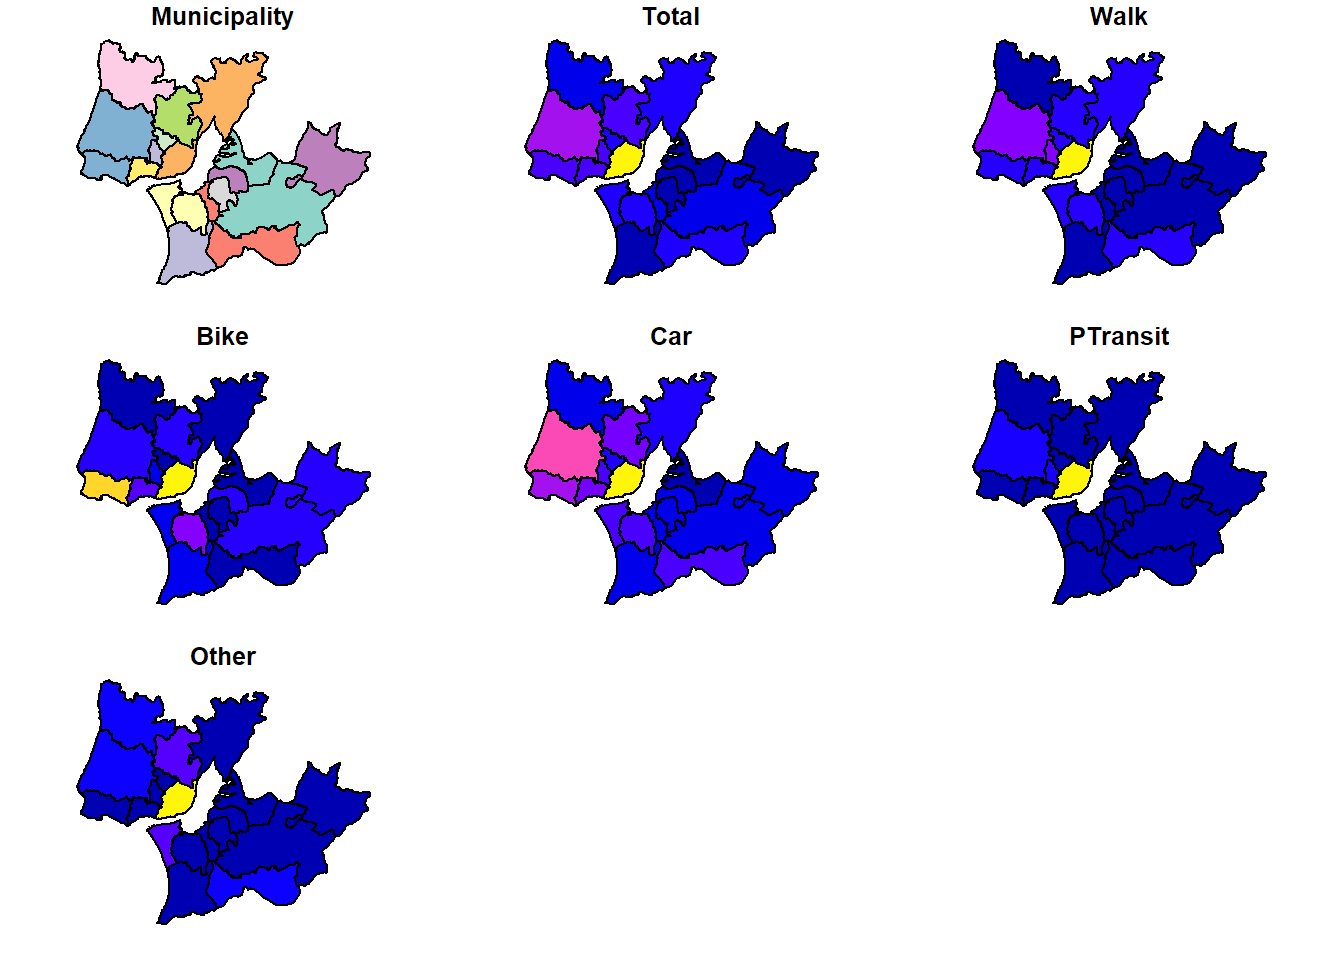
\includegraphics{interactive-maps_files/figure-pdf/unnamed-chunk-2-1.pdf}

Interactive maps are useful to explore the data, as you can zoom in and
out, and click on the points to see the data associated with them.

There are several R packages to create interactive maps. For instance,
the \texttt{tmap} package, the \texttt{leaflet} package, and the
\texttt{mapview} package.

\section{Mapview}\label{mapview}

Mapview allows to create quick interactive maps, only by declaring the
function \texttt{mapview()}.

\begin{Shaded}
\begin{Highlighting}[]
\FunctionTok{library}\NormalTok{(mapview)}
\FunctionTok{mapview}\NormalTok{(TRIPSgeo)}
\end{Highlighting}
\end{Shaded}

\includegraphics{interactive-maps_files/figure-pdf/unnamed-chunk-3-1.png}

To color the points by a variable, you can use the \texttt{zcol}
argument.

\begin{Shaded}
\begin{Highlighting}[]
\FunctionTok{mapview}\NormalTok{(TRIPSgeo, }\AttributeTok{zcol =} \StringTok{"Total"}\NormalTok{)}
\end{Highlighting}
\end{Shaded}

\includegraphics{interactive-maps_files/figure-pdf/unnamed-chunk-4-1.png}

As you can see, a color palette is automatically assigned to the
\textbf{continuous variable}.

Try to use a \textbf{categorical variable}.

\begin{Shaded}
\begin{Highlighting}[]
\FunctionTok{mapview}\NormalTok{(TRIPSgeo, }\AttributeTok{zcol =} \StringTok{"Municipality"}\NormalTok{, }\AttributeTok{alpha.regions =} \FloatTok{0.4}\NormalTok{) }\CommentTok{\# also add transparency)}
\end{Highlighting}
\end{Shaded}

\begin{tcolorbox}[enhanced jigsaw, breakable, left=2mm, colframe=quarto-callout-note-color-frame, leftrule=.75mm, bottomrule=.15mm, arc=.35mm, rightrule=.15mm, colback=white, opacityback=0, toprule=.15mm]
\begin{minipage}[t]{5.5mm}
\textcolor{quarto-callout-note-color}{\faInfo}
\end{minipage}%
\begin{minipage}[t]{\textwidth - 5.5mm}

Note that you can change the \textbf{basemap}, and click on the
geometries to \textbf{see the data} associated with them.

\end{minipage}%
\end{tcolorbox}

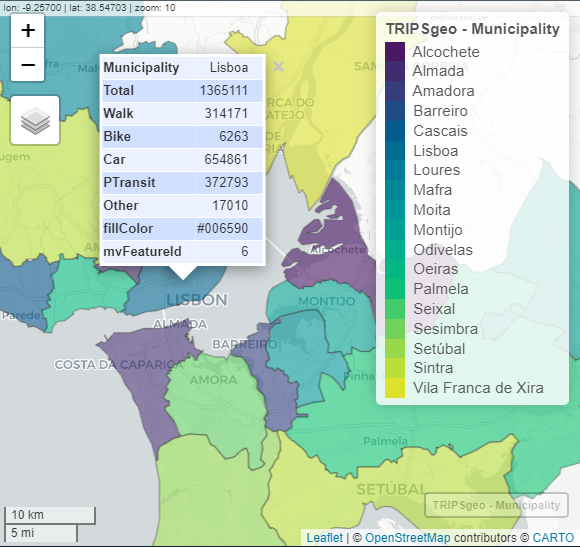
\includegraphics[width=5.625in,height=\textheight]{images/clipboard-3307189144.png}

You can go crazy with all the options that \texttt{mapview} offers.
Please refer to the
\href{https://r-spatial.github.io/mapview/articles/mapview_02-advanced.html}{documentation}
to see all the options.

\subsection{Export}\label{export}

You can directly export the map as an \texttt{html} file or image, using
the Viewer panel.

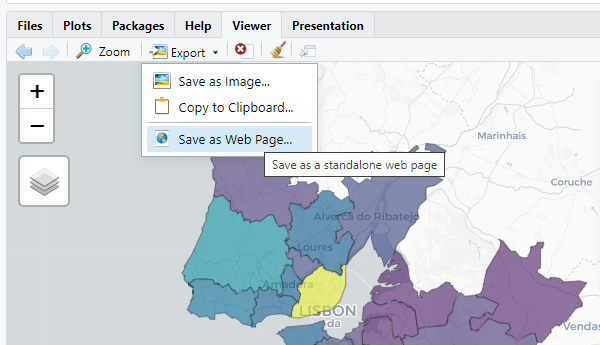
\includegraphics[width=4.89583in,height=\textheight]{images/clipboard-3542861620.png}

\begin{tcolorbox}[enhanced jigsaw, breakable, left=2mm, colframe=quarto-callout-warning-color-frame, leftrule=.75mm, bottomrule=.15mm, arc=.35mm, rightrule=.15mm, colback=white, opacityback=0, toprule=.15mm]

This is the most straightforward solution.

\end{tcolorbox}

You can also export a map as an html file or image using code.

\begin{Shaded}
\begin{Highlighting}[]
\CommentTok{\# install.packages("webshot2") \# you will need this}

\NormalTok{map }\OtherTok{=} \FunctionTok{mapview}\NormalTok{(TRIPSgeo, }\AttributeTok{zcol =} \StringTok{"Total"}\NormalTok{) }\CommentTok{\# fisrt create a objet with the desired map}

\FunctionTok{mapshot2}\NormalTok{(map, }\StringTok{"data/map.html"}\NormalTok{) }\CommentTok{\# as webpage}
\FunctionTok{mapshot2}\NormalTok{(map, }\AttributeTok{file =} \StringTok{"data/map.png"}\NormalTok{) }\CommentTok{\# as image}
\end{Highlighting}
\end{Shaded}

\section{Rmarkdown}\label{rmarkdown}

To include a map on a report, website, paper (any type), you can create
an Rmarkdown file.

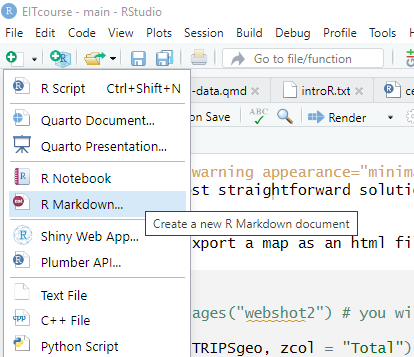
\includegraphics[width=4.04167in,height=\textheight]{images/clipboard-1842640045.png}

And include a R code chunk (\texttt{ctrl\ +\ alt\ +\ i}) with a map. If
the output is html, you will get an interactive map on your document!

\part{\textbf{Day 2}}

\chapter{Centroids of transport
zones}\label{centroids-of-transport-zones}

In this section we will calculate the geometric and the weighted
centroids of transport zones.

\section{Geometric centroids}\label{geometric-centroids}

Taking the \texttt{Municipalities\_geo} data from the previous section,
we will calculate the geometric centroids, using the
\texttt{st\_centroid()} function.

\begin{Shaded}
\begin{Highlighting}[]
\FunctionTok{library}\NormalTok{(dplyr)}
\FunctionTok{library}\NormalTok{(sf)}
\FunctionTok{library}\NormalTok{(mapview)}

\NormalTok{Municipalities\_geo }\OtherTok{=} \FunctionTok{st\_read}\NormalTok{(}\StringTok{"data/Municipalities\_geo.gpkg"}\NormalTok{, }\AttributeTok{quiet =} \ConstantTok{TRUE}\NormalTok{)}

\NormalTok{Centroids\_geo }\OtherTok{=} \FunctionTok{st\_centroid}\NormalTok{(Municipalities\_geo)}
\end{Highlighting}
\end{Shaded}

This creates points at the geometric center of each polygon.

\begin{Shaded}
\begin{Highlighting}[]
\FunctionTok{mapview}\NormalTok{(Centroids\_geo)}
\end{Highlighting}
\end{Shaded}

\includegraphics{centroids_files/figure-pdf/unnamed-chunk-1-1.png}

\begin{Shaded}
\begin{Highlighting}[]
\FunctionTok{mapview}\NormalTok{(Centroids\_geo) }\SpecialCharTok{+} \FunctionTok{mapview}\NormalTok{(Municipalities\_geo, }\AttributeTok{alpha.regions =} \DecValTok{0}\NormalTok{) }\CommentTok{\# both maps, with full transparency in polygons}
\end{Highlighting}
\end{Shaded}

\includegraphics{centroids_files/figure-pdf/unnamed-chunk-1-2.png}

But\ldots{} is this the best way to represent the center of a transport
zone?

These results may be biased by the shape of the polygons, and not
represent where activities are. Example: lakes, forests, etc.

To overcome this, we can use \textbf{weighted centroids}.

\section{Weighted centroids}\label{weighted-centroids}

We will weight centroids of transport zones by population and by number
of buildings.

For this, we will need the census data (INE 2022).

\begin{Shaded}
\begin{Highlighting}[]
\NormalTok{Census }\OtherTok{=} \FunctionTok{st\_read}\NormalTok{(}\StringTok{"data/census.gpkg"}\NormalTok{, }\AttributeTok{quiet =} \ConstantTok{TRUE}\NormalTok{)}

\FunctionTok{mapview}\NormalTok{(Census }\SpecialCharTok{|\textgreater{}} \FunctionTok{filter}\NormalTok{(Municipality }\SpecialCharTok{==} \StringTok{"Lisboa"}\NormalTok{), }\AttributeTok{zcol =} \StringTok{"Population"}\NormalTok{)}
\end{Highlighting}
\end{Shaded}

\includegraphics{centroids_files/figure-pdf/getcensus-1.png}

It was not that easy to estimate weighted centroids with R, as it is
with GIS software. But there is this new package
\href{https://ryanzomorrodi.github.io/centr}{\texttt{centr}} that can
help us (Zomorrodi 2024).

We need to specify the \textbf{group} we want to calculate the
\textbf{mean centroids}, and the \textbf{weight variable} we want to
use.

\begin{Shaded}
\begin{Highlighting}[]
\CommentTok{\# test}
\FunctionTok{library}\NormalTok{(centr)}
\NormalTok{Centroid\_pop }\OtherTok{=}\NormalTok{ Census }\SpecialCharTok{|\textgreater{}} 
  \FunctionTok{mean\_center}\NormalTok{(}\AttributeTok{group =} \StringTok{"Municipality"}\NormalTok{, }\AttributeTok{weight =} \StringTok{"Population"}\NormalTok{)}
\end{Highlighting}
\end{Shaded}

We can do the same for buildings.

\begin{Shaded}
\begin{Highlighting}[]
\NormalTok{Centroid\_build }\OtherTok{=}\NormalTok{ Census }\SpecialCharTok{|\textgreater{}} 
  \FunctionTok{mean\_center}\NormalTok{(}\AttributeTok{group =} \StringTok{"Municipality"}\NormalTok{, }\AttributeTok{weight =} \StringTok{"Buildings"}\NormalTok{)}
\end{Highlighting}
\end{Shaded}

\section{Compare centroids in a map}\label{compare-centroids-in-a-map}

\subsection{Interactive map}\label{interactive-map}

\begin{Shaded}
\begin{Highlighting}[]
\FunctionTok{mapview}\NormalTok{(Centroids\_geo, }\AttributeTok{col.region =} \StringTok{"blue"}\NormalTok{) }\SpecialCharTok{+}
  \FunctionTok{mapview}\NormalTok{(Centroid\_pop, }\AttributeTok{col.region =} \StringTok{"red"}\NormalTok{) }\SpecialCharTok{+}
  \FunctionTok{mapview}\NormalTok{(Centroid\_build, }\AttributeTok{col.region =} \StringTok{"black"}\NormalTok{) }\SpecialCharTok{+}
  \FunctionTok{mapview}\NormalTok{(Municipalities\_geo, }\AttributeTok{alpha.regions =} \DecValTok{0}\NormalTok{) }\CommentTok{\# polygon limits}
\end{Highlighting}
\end{Shaded}

\includegraphics{centroids_files/figure-pdf/unnamed-chunk-5-1.png}

See how the building, population and geometric centroids of Sintra are
apart, from closer to Tagus, to the rural area.

\subsection{Static map}\label{static-map}

To produce the same map, using only \texttt{plot()} and
\texttt{st\_geometry()}, we need to make sure that the geometries have
the same crs.

\begin{Shaded}
\begin{Highlighting}[]
\FunctionTok{st\_crs}\NormalTok{(Centroids\_geo) }\CommentTok{\# 4326 WGS84}
\FunctionTok{st\_crs}\NormalTok{(Centroid\_pop) }\CommentTok{\# 3763 Portugal TM06}
\end{Highlighting}
\end{Shaded}

So, we need to transform the geometries to the same crs.

\begin{Shaded}
\begin{Highlighting}[]
\NormalTok{Centroid\_pop }\OtherTok{=} \FunctionTok{st\_transform}\NormalTok{(Centroid\_pop, }\AttributeTok{crs =} \DecValTok{4326}\NormalTok{)}
\NormalTok{Centroid\_build }\OtherTok{=} \FunctionTok{st\_transform}\NormalTok{(Centroid\_build, }\AttributeTok{crs =} \DecValTok{4326}\NormalTok{)}
\end{Highlighting}
\end{Shaded}

Now, to use \texttt{plot()} we incrementally add layers to the plot.

\begin{Shaded}
\begin{Highlighting}[]
\CommentTok{\# Plot the Municipalities\_geo polygons first (with no fill)}
\FunctionTok{plot}\NormalTok{(}\FunctionTok{st\_geometry}\NormalTok{(Municipalities\_geo), }\AttributeTok{col =} \ConstantTok{NA}\NormalTok{, }\AttributeTok{border =} \StringTok{"black"}\NormalTok{, }\AttributeTok{main =} \StringTok{"Map of different Centroids of Municipalities"}\NormalTok{)}

\CommentTok{\# Add the Centroids\_geo points in blue}
\FunctionTok{plot}\NormalTok{(}\FunctionTok{st\_geometry}\NormalTok{(Centroids\_geo), }\AttributeTok{col =} \StringTok{"blue"}\NormalTok{, }\AttributeTok{pch =} \DecValTok{16}\NormalTok{, }\AttributeTok{add =} \ConstantTok{TRUE}\NormalTok{) }\CommentTok{\# add!}

\CommentTok{\# Add the Centroid\_pop points in red}
\FunctionTok{plot}\NormalTok{(}\FunctionTok{st\_geometry}\NormalTok{(Centroid\_pop), }\AttributeTok{col =} \StringTok{"red"}\NormalTok{, }\AttributeTok{pch =} \DecValTok{16}\NormalTok{, }\AttributeTok{add =} \ConstantTok{TRUE}\NormalTok{)}

\CommentTok{\# Add the Centroid\_build points in black}
\FunctionTok{plot}\NormalTok{(}\FunctionTok{st\_geometry}\NormalTok{(Centroid\_build), }\AttributeTok{col =} \StringTok{"black"}\NormalTok{, }\AttributeTok{pch =} \DecValTok{16}\NormalTok{, }\AttributeTok{add =} \ConstantTok{TRUE}\NormalTok{)}
\end{Highlighting}
\end{Shaded}

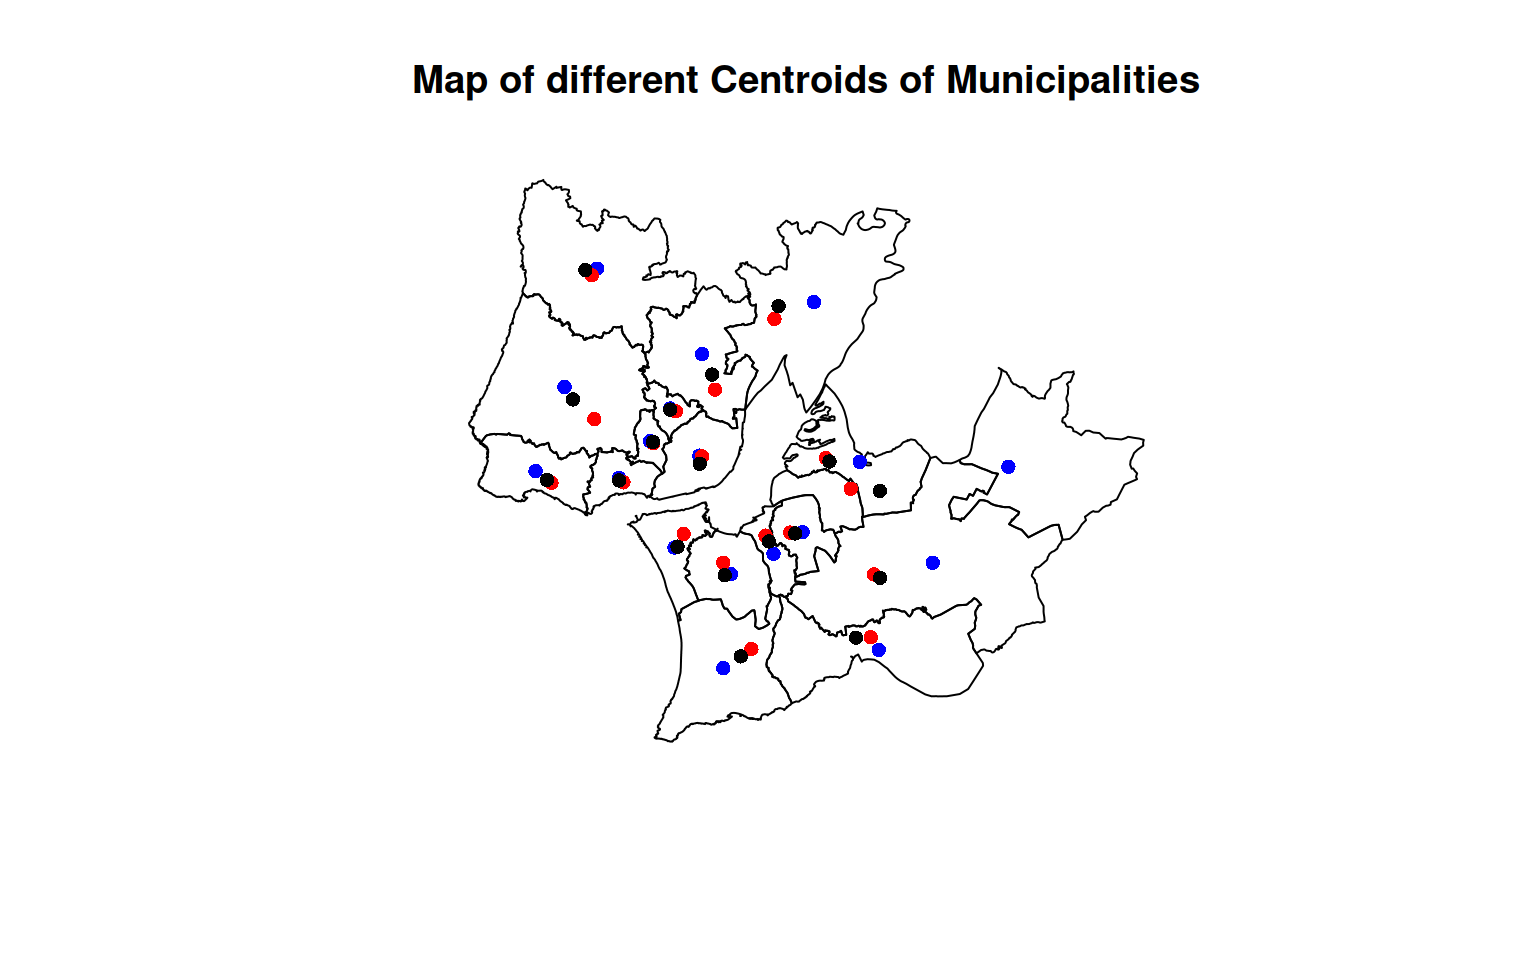
\includegraphics{centroids_files/figure-pdf/unnamed-chunk-8-1.pdf}

In the next section we will use these centroids to calculate the desire
lines between them.

\chapter{OD pairs and desire lines}\label{od-pairs-and-desire-lines}

Desire lines are a way to represent the flow of people or goods between
two points. They are often used in transport planning to represent the
flow of trips between zones.

The
\href{https://docs.ropensci.org/stplanr/index.html}{\texttt{stplanr}}
package is a collection of functions for sustainable transport planning
with R, and it is built on top of the \texttt{sf} package (Lovelace and
Ellison 2018).

In this workshop, we will use the
\href{https://itsleeds.github.io/od/}{\texttt{od}} package, a
lightweight package with a few functions from \texttt{stplanr}, namely
the ones to create desire lines from origin-destination (OD) pairs
(Lovelace and Morgan 2024).

\section{Desire lines with od\_2\_sf}\label{desire-lines-with-od_2_sf}

To create desire lines, we need a dataset with OD pairs \textbf{and}
other dataset with the corresponding transport zones (spatial data).

The \texttt{TRIPSmode.Rds} dataset includes origins, destinations and
number of trips between municipalities.

\begin{Shaded}
\begin{Highlighting}[]
\NormalTok{TRIPSmode }\OtherTok{=} \FunctionTok{readRDS}\NormalTok{(}\StringTok{"data/TRIPSmode.Rds"}\NormalTok{)}
\end{Highlighting}
\end{Shaded}

The \texttt{Municipalities\_geo.gpkg} dataset includes the geometry of
the transport zones.

\begin{Shaded}
\begin{Highlighting}[]
\FunctionTok{library}\NormalTok{(sf)}
\NormalTok{Municipalities\_geo }\OtherTok{=} \FunctionTok{st\_read}\NormalTok{(}\StringTok{"data/Municipalities\_geo.gpkg"}\NormalTok{, }\AttributeTok{quiet =} \ConstantTok{TRUE}\NormalTok{) }\CommentTok{\# supress mesage}
\end{Highlighting}
\end{Shaded}

Then, we need to load the \texttt{od} package. We will use the
\texttt{od\_to\_sf()} function to create desire lines from OD pairs.

\begin{Shaded}
\begin{Highlighting}[]
\CommentTok{\# install.packages("od")}
\FunctionTok{library}\NormalTok{(od)}

\NormalTok{TRIPSdlines }\OtherTok{=} \FunctionTok{od\_to\_sf}\NormalTok{(TRIPSmode, }\AttributeTok{z =}\NormalTok{ Municipalities\_geo) }\CommentTok{\# z for zones}
\end{Highlighting}
\end{Shaded}

For this magic to work smoothly, the first two columns of the
\texttt{TRIPSmode} dataset must be the \textbf{origin} and
\textbf{destination} zones, and these zones need to correspond to the
first column of the \texttt{Municipalities\_geo} dataset (with an
associated geometry).

\begin{tcolorbox}[enhanced jigsaw, breakable, left=2mm, colframe=quarto-callout-tip-color-frame, leftrule=.75mm, bottomrule=.15mm, arc=.35mm, rightrule=.15mm, colback=white, opacityback=0, toprule=.15mm]

See more options with the \texttt{?stplanr::od2line} function.

\end{tcolorbox}

Now we can visualize the desire lines using the \texttt{mapview}
function.

\begin{Shaded}
\begin{Highlighting}[]
\FunctionTok{library}\NormalTok{(mapview)}
\FunctionTok{mapview}\NormalTok{(TRIPSdlines, }\AttributeTok{zcol =} \StringTok{"Total"}\NormalTok{)}
\end{Highlighting}
\end{Shaded}

\includegraphics{desire-lines_files/figure-pdf/unnamed-chunk-4-1.png}

As you can see, this is too much information to be able to understand
the flows.

\subsection{Filtering desire lines}\label{filtering-desire-lines}

Filter \textbf{intrazonal} trips.

\begin{Shaded}
\begin{Highlighting}[]
\FunctionTok{library}\NormalTok{(dplyr)}

\NormalTok{TRIPSdlines\_inter }\OtherTok{=}\NormalTok{ TRIPSdlines }\SpecialCharTok{|\textgreater{}} 
  \FunctionTok{filter}\NormalTok{(Origin }\SpecialCharTok{!=}\NormalTok{ Destination) }\SpecialCharTok{|\textgreater{}} \CommentTok{\# remove intrazonal trips}
  \FunctionTok{filter}\NormalTok{(Total }\SpecialCharTok{\textgreater{}} \DecValTok{5000}\NormalTok{) }\CommentTok{\# remove noise}

\FunctionTok{mapview}\NormalTok{(TRIPSdlines\_inter, }\AttributeTok{zcol =} \StringTok{"Total"}\NormalTok{, }\AttributeTok{lwd =} \DecValTok{5}\NormalTok{)}
\end{Highlighting}
\end{Shaded}

\includegraphics{desire-lines_files/figure-pdf/unnamed-chunk-5-1.png}

Filter trips with origin or destination \textbf{not in} Lisbon.

\begin{Shaded}
\begin{Highlighting}[]
\NormalTok{TRIPSdl\_noLX }\OtherTok{=}\NormalTok{ TRIPSdlines\_inter }\SpecialCharTok{|\textgreater{}} 
  \FunctionTok{filter}\NormalTok{(Origin }\SpecialCharTok{!=} \StringTok{"Lisboa"}\NormalTok{, Destination }\SpecialCharTok{!=} \StringTok{"Lisboa"}\NormalTok{)}

\FunctionTok{mapview}\NormalTok{(TRIPSdl\_noLX, }\AttributeTok{zcol =} \StringTok{"Total"}\NormalTok{, }\AttributeTok{lwd =} \DecValTok{8}\NormalTok{) }\CommentTok{\# larger line width}
\end{Highlighting}
\end{Shaded}

\includegraphics{desire-lines_files/figure-pdf/unnamed-chunk-6-1.png}

Try to replace the \texttt{Total} with other variables, such as
\texttt{Car}, \texttt{PTransit}, and see the differences.

\section{Oneway desire lines}\label{oneway-desire-lines}

Note that the \texttt{od\_to\_sf()} function creates bidirectional
desire lines. This can be not the ideal for visualization /
representation purposes, as you will have 2 lines overlaping.

The function
\href{https://itsleeds.github.io/od/reference/od_oneway.html}{\texttt{od\_oneway()}}
aggregates oneway lines to produce bidirectional flows.

By default, it returns the sum of each numeric column for each
bidirectional origin-destination pair.

\begin{Shaded}
\begin{Highlighting}[]
\FunctionTok{nrow}\NormalTok{(TRIPSdlines)}
\end{Highlighting}
\end{Shaded}

\begin{verbatim}
[1] 315
\end{verbatim}

\begin{Shaded}
\begin{Highlighting}[]
\NormalTok{TRIPSdlines\_oneway }\OtherTok{=} \FunctionTok{od\_oneway}\NormalTok{(TRIPSdlines)}
\FunctionTok{nrow}\NormalTok{(TRIPSdlines\_oneway)}
\end{Highlighting}
\end{Shaded}

\begin{verbatim}
[1] 168
\end{verbatim}

Note that for the last municipalities you have less combinations now.
Nevertheless, all the possible combinations are represented.

\begin{Shaded}
\begin{Highlighting}[]
\FunctionTok{head}\NormalTok{(TRIPSdlines\_oneway[,}\FunctionTok{c}\NormalTok{(}\DecValTok{1}\NormalTok{,}\DecValTok{2}\NormalTok{)]) }\CommentTok{\# just the first 2 columns}
\end{Highlighting}
\end{Shaded}

\begin{verbatim}
Simple feature collection with 6 features and 2 fields
Attribute-geometry relationships: identity (2) (with 3 geometries empty)
Geometry type: LINESTRING
Dimension:     XY
Bounding box:  xmin: -9.229502 ymin: 38.63562 xmax: -8.91588 ymax: 38.75981
Geodetic CRS:  WGS 84
          o         d                       geometry
1 Alcochete Alcochete               LINESTRING EMPTY
2 Alcochete    Almada LINESTRING (-8.91588 38.735...
3    Almada    Almada               LINESTRING EMPTY
4 Alcochete   Amadora LINESTRING (-8.91588 38.735...
5    Almada   Amadora LINESTRING (-9.193069 38.63...
6   Amadora   Amadora               LINESTRING EMPTY
\end{verbatim}

\begin{Shaded}
\begin{Highlighting}[]
\FunctionTok{tail}\NormalTok{(TRIPSdlines\_oneway[,}\FunctionTok{c}\NormalTok{(}\DecValTok{1}\NormalTok{,}\DecValTok{2}\NormalTok{)])}
\end{Highlighting}
\end{Shaded}

\begin{verbatim}
Simple feature collection with 6 features and 2 fields
Attribute-geometry relationships: identity (2) (with 1 geometry empty)
Geometry type: LINESTRING
Dimension:     XY
Bounding box:  xmin: -9.357651 ymin: 38.4949 xmax: -8.806644 ymax: 38.92211
Geodetic CRS:  WGS 84
                      o                   d                       geometry
163             Palmela Vila Franca de Xira LINESTRING (-8.806644 38.61...
164              Seixal Vila Franca de Xira LINESTRING (-9.108801 38.60...
165            Sesimbra Vila Franca de Xira LINESTRING (-9.120124 38.49...
166             Setúbal Vila Franca de Xira LINESTRING (-8.887481 38.51...
167              Sintra Vila Franca de Xira LINESTRING (-9.357651 38.82...
168 Vila Franca de Xira Vila Franca de Xira               LINESTRING EMPTY
\end{verbatim}

Example of visualization with Public Transit trips in both ways.

\begin{Shaded}
\begin{Highlighting}[]
\NormalTok{TRIPSdlines\_oneway\_noLX }\OtherTok{=}\NormalTok{ TRIPSdlines\_oneway }\SpecialCharTok{|\textgreater{}} 
  \FunctionTok{filter}\NormalTok{(o }\SpecialCharTok{!=}\NormalTok{ d) }\SpecialCharTok{|\textgreater{}} \CommentTok{\# remove intrazonal trips}
  \FunctionTok{filter}\NormalTok{(PTransit }\SpecialCharTok{\textgreater{}} \DecValTok{5000}\NormalTok{) }\CommentTok{\# reduce noise}

\FunctionTok{mapview}\NormalTok{(TRIPSdlines\_oneway\_noLX, }\AttributeTok{zcol =} \StringTok{"PTransit"}\NormalTok{, }\AttributeTok{lwd =} \DecValTok{8}\NormalTok{)}
\end{Highlighting}
\end{Shaded}

\includegraphics{desire-lines_files/figure-pdf/unnamed-chunk-9-1.png}

\section{Using population centroids}\label{using-population-centroids}

The \texttt{od\_to\_sf()} function uses the geometric center of the
zones to create the desire lines. But if we replace those zones by the
\hyperref[weighted-centroids]{weighted centroids}, we can have a more
realistic representation of the flows.

\begin{Shaded}
\begin{Highlighting}[]
\CommentTok{\# Centroid\_pop = st\_read("data/Centroid\_pop.gpkg")}

\NormalTok{TRIPSdlines\_pop }\OtherTok{=} \FunctionTok{od\_to\_sf}\NormalTok{(TRIPSmode, }\AttributeTok{z =}\NormalTok{ Centroid\_pop) }\SpecialCharTok{|\textgreater{}}  \CommentTok{\# works the same way}
  \FunctionTok{od\_oneway}\NormalTok{() }\CommentTok{\# oneway}
\end{Highlighting}
\end{Shaded}

Check differences of lines with trips from/to Lisbon:

\begin{Shaded}
\begin{Highlighting}[]
\NormalTok{TRIPSdlines\_geo\_LX }\OtherTok{=}\NormalTok{ TRIPSdlines\_oneway }\SpecialCharTok{|\textgreater{}} 
  \FunctionTok{filter}\NormalTok{(o }\SpecialCharTok{==} \StringTok{"Lisboa"} \SpecialCharTok{|}\NormalTok{ d }\SpecialCharTok{==} \StringTok{"Lisboa"}\NormalTok{) }\CommentTok{\# or condition}
\NormalTok{TRIPSdlines\_pop\_LX }\OtherTok{=}\NormalTok{ TRIPSdlines\_pop }\SpecialCharTok{|\textgreater{}} 
  \FunctionTok{filter}\NormalTok{(o }\SpecialCharTok{==} \StringTok{"Lisboa"} \SpecialCharTok{|}\NormalTok{ d }\SpecialCharTok{==} \StringTok{"Lisboa"}\NormalTok{)}

\FunctionTok{mapview}\NormalTok{(TRIPSdlines\_geo\_LX, }\AttributeTok{color =} \StringTok{"blue"}\NormalTok{) }\SpecialCharTok{+} \FunctionTok{mapview}\NormalTok{(TRIPSdlines\_pop\_LX, }\AttributeTok{color =} \StringTok{"red"}\NormalTok{)}
\end{Highlighting}
\end{Shaded}

\includegraphics{desire-lines_files/figure-pdf/unnamed-chunk-12-1.png}

The next step will be estimating the \textbf{euclidean distances}
between these centroids, and compare them with the \textbf{routing
distances}.

\chapter{Euclidean and routing
distances}\label{euclidean-and-routing-distances}

We will show how to estimate euclidean distances (\emph{as crown
flights}) using \texttt{sf} package, and the distances using a road
network using \texttt{r5r} package (demonstrative).

\section{Euclidean distances}\label{euclidean-distances}

Taking the survey respondents' location, we will estimate the distance
to the university (IST) using the \texttt{sf} package.

\subsection{Import survey data frame convert to
sf}\label{import-survey-data-frame-convert-to-sf}

We will use a survey dataset with 200 observations, with the following
variables: ID, Affiliation, Age, Sex, Transport Mode to IST, and
latitude and longitude coordinates.

\begin{Shaded}
\begin{Highlighting}[]
\FunctionTok{library}\NormalTok{(dplyr)}

\NormalTok{SURVEY }\OtherTok{=} \FunctionTok{read.csv}\NormalTok{(}\StringTok{"data/SURVEY.txt"}\NormalTok{, }\AttributeTok{sep =} \StringTok{"}\SpecialCharTok{\textbackslash{}t}\StringTok{"}\NormalTok{) }\CommentTok{\# tab delimiter}
\FunctionTok{names}\NormalTok{(SURVEY)}
\end{Highlighting}
\end{Shaded}

\begin{verbatim}
[1] "ID"   "AFF"  "AGE"  "SEX"  "MODE" "lat"  "lon" 
\end{verbatim}

As we have the coordinates, we can convert this data frame to a spatial
feature, as explained in the
\hyperref[create-spatial-data-from-coordinates]{Introduction to spatial
data} section.

\begin{Shaded}
\begin{Highlighting}[]
\FunctionTok{library}\NormalTok{(sf)}

\NormalTok{SURVEYgeo }\OtherTok{=} \FunctionTok{st\_as\_sf}\NormalTok{(SURVEY, }\AttributeTok{coords =} \FunctionTok{c}\NormalTok{(}\StringTok{"lon"}\NormalTok{, }\StringTok{"lat"}\NormalTok{), }\AttributeTok{crs =} \DecValTok{4326}\NormalTok{) }\CommentTok{\# convert to as sf data}
\end{Highlighting}
\end{Shaded}

\subsection{Create new point at the
university}\label{create-new-point-at-the-university}

Using coordinates from Instituto Superior Técnico, we can directly
create a simple feature and assign its crs.

\begin{Shaded}
\begin{Highlighting}[]
\NormalTok{UNIVERSITY }\OtherTok{=} \FunctionTok{data.frame}\NormalTok{(}\AttributeTok{place =} \StringTok{"IST"}\NormalTok{,}
                        \AttributeTok{lon =} \SpecialCharTok{{-}}\FloatTok{9.1397404}\NormalTok{,}
                        \AttributeTok{lat =} \FloatTok{38.7370168}\NormalTok{) }\SpecialCharTok{|\textgreater{}}  \CommentTok{\# first a dataframe}
  \FunctionTok{st\_as\_sf}\NormalTok{(}\AttributeTok{coords =} \FunctionTok{c}\NormalTok{(}\StringTok{"lon"}\NormalTok{, }\StringTok{"lat"}\NormalTok{), }\CommentTok{\# then a spacial feature}
           \AttributeTok{crs =} \DecValTok{4326}\NormalTok{)}
\end{Highlighting}
\end{Shaded}

Visualize in a map:

\begin{Shaded}
\begin{Highlighting}[]
\FunctionTok{library}\NormalTok{(mapview)}
\FunctionTok{mapview}\NormalTok{(SURVEYgeo, }\AttributeTok{zcol =} \StringTok{"MODE"}\NormalTok{) }\SpecialCharTok{+} \FunctionTok{mapview}\NormalTok{(UNIVERSITY, }\AttributeTok{col.region =} \StringTok{"red"}\NormalTok{, }\AttributeTok{cex =} \DecValTok{12}\NormalTok{)}
\end{Highlighting}
\end{Shaded}

\includegraphics{distances_files/figure-pdf/unnamed-chunk-4-1.png}

\subsection{Straight lines}\label{straight-lines}

First we will create lines connecting the survey locations to the
university, using the \texttt{st\_nearest\_points()} function.

This function finds returns the nearest points between two geometries,
and creates a line between them. This can be useful to find the nearest
train station to each point, for instance.

As we only have 1 point at UNIVERSITY layer, we will have the same
number of lines as number of surveys = 200.

\begin{Shaded}
\begin{Highlighting}[]
\NormalTok{SURVEYeuclidean }\OtherTok{=} \FunctionTok{st\_nearest\_points}\NormalTok{(SURVEYgeo, UNIVERSITY, }\AttributeTok{pairwise =} \ConstantTok{TRUE}\NormalTok{) }\SpecialCharTok{|\textgreater{}}
  \FunctionTok{st\_as\_sf}\NormalTok{() }\CommentTok{\# this creates lines}

\FunctionTok{mapview}\NormalTok{(SURVEYeuclidean)}
\end{Highlighting}
\end{Shaded}

\begin{verbatim}
Warning in cbind(`Feature ID` = fid, mat): number of rows of result is not a
multiple of vector length (arg 1)
\end{verbatim}

\includegraphics{distances_files/figure-pdf/unnamed-chunk-5-1.png}

Note that if we have more than one point in the second layer, the
\texttt{pairwise\ =\ TRUE} will create a line for each combination of
points. Set to \texttt{FALSE} if, for instance, you have the same number
of points in both layers and want to create a line between the
corresponding points.

\subsection{Distance}\label{distance}

Now we can estimate the distance using the \texttt{st\_length()}
function.

\begin{Shaded}
\begin{Highlighting}[]
\CommentTok{\# compute the line length and add directly in the first survey layer}
\NormalTok{SURVEYgeo }\OtherTok{=}\NormalTok{ SURVEYgeo }\SpecialCharTok{|\textgreater{}} 
  \FunctionTok{mutate}\NormalTok{(}\AttributeTok{distance =} \FunctionTok{st\_length}\NormalTok{(SURVEYeuclidean))}

\CommentTok{\# remove the units {-} can be useful}
\NormalTok{SURVEYgeo}\SpecialCharTok{$}\NormalTok{distance }\OtherTok{=}\NormalTok{ units}\SpecialCharTok{::}\FunctionTok{drop\_units}\NormalTok{(SURVEYgeo}\SpecialCharTok{$}\NormalTok{distance) }
\end{Highlighting}
\end{Shaded}

We could also estimate the distance using the \texttt{st\_distance()}
function \textbf{directly}, without creating the lines.

\begin{Shaded}
\begin{Highlighting}[]
\NormalTok{SURVEYgeo }\OtherTok{=}\NormalTok{ SURVEYgeo }\SpecialCharTok{|\textgreater{}} 
  \FunctionTok{mutate}\NormalTok{(}\AttributeTok{distance =} \FunctionTok{st\_distance}\NormalTok{(SURVEYgeo, UNIVERSITY)[,}\DecValTok{1}\NormalTok{] }\SpecialCharTok{|\textgreater{}}  \CommentTok{\# in meters}
\NormalTok{           units}\SpecialCharTok{::}\FunctionTok{drop\_units}\NormalTok{()) }\SpecialCharTok{|\textgreater{}}  \CommentTok{\# remove units}
  \FunctionTok{mutate}\NormalTok{(}\AttributeTok{distance =} \FunctionTok{round}\NormalTok{(distance)) }\CommentTok{\# round to integer}

\FunctionTok{summary}\NormalTok{(SURVEYgeo}\SpecialCharTok{$}\NormalTok{distance)}
\end{Highlighting}
\end{Shaded}

\begin{verbatim}
   Min. 1st Qu.  Median    Mean 3rd Qu.    Max. 
    298    1106    2186    2658    3683    8600 
\end{verbatim}

\section{Routing distances with r5r}\label{routing-distances-with-r5r}

We use the \texttt{r5r} package to estimate the distance using a road
network.

\begin{tcolorbox}[enhanced jigsaw, breakable, left=2mm, colframe=quarto-callout-note-color-frame, leftrule=.75mm, bottomrule=.15mm, arc=.35mm, rightrule=.15mm, colback=white, opacityback=0, toprule=.15mm]
\begin{minipage}[t]{5.5mm}
\textcolor{quarto-callout-note-color}{\faInfo}
\end{minipage}%
\begin{minipage}[t]{\textwidth - 5.5mm}

To properly the setup r5r model for the area you are working on, you
need to download the \textbf{road network} data from OpenStreetMap and,
if needed, add a \textbf{GTFS} and \textbf{DEM} file, as it will be
explained in the \href{r5r.qmd}{next section}.

\end{minipage}%
\end{tcolorbox}

We will use only respondents with a distance to the university less than
2 km.

\begin{Shaded}
\begin{Highlighting}[]
\NormalTok{SURVEYsample }\OtherTok{=}\NormalTok{ SURVEYgeo }\SpecialCharTok{|\textgreater{}} \FunctionTok{filter}\NormalTok{(distance }\SpecialCharTok{\textless{}=} \DecValTok{2000}\NormalTok{)}
\FunctionTok{nrow}\NormalTok{(SURVEYsample)}
\end{Highlighting}
\end{Shaded}

\begin{verbatim}
[1] 95
\end{verbatim}

We need an id (unique identifier) for each survey location, to be used
in the routing functions of \texttt{r5r}.

\begin{Shaded}
\begin{Highlighting}[]
\CommentTok{\# create id columns for both datasets}
\NormalTok{SURVEYsample }\OtherTok{=}\NormalTok{ SURVEYsample }\SpecialCharTok{|\textgreater{}} 
  \FunctionTok{mutate}\NormalTok{(}\AttributeTok{id =} \FunctionTok{c}\NormalTok{(}\DecValTok{1}\SpecialCharTok{:}\FunctionTok{nrow}\NormalTok{(SURVEYsample))) }\CommentTok{\# from 1 to the number of rows}

\NormalTok{UNIVERSITY }\OtherTok{=}\NormalTok{ UNIVERSITY }\SpecialCharTok{|\textgreater{}} 
  \FunctionTok{mutate}\NormalTok{(}\AttributeTok{id =} \DecValTok{1}\NormalTok{) }\CommentTok{\# only one row}
\end{Highlighting}
\end{Shaded}

\subsection{Distances by car}\label{distances-by-car}

Estimate the routes with time and distance by car, from survey locations
to University.

\begin{Shaded}
\begin{Highlighting}[]
\NormalTok{SURVEYcar }\OtherTok{=} \FunctionTok{detailed\_itineraries}\NormalTok{(}
  \AttributeTok{r5r\_core =}\NormalTok{ r5r\_network,}
  \AttributeTok{origins =}\NormalTok{ SURVEYsample,}
  \AttributeTok{destinations =}\NormalTok{ UNIVERSITY,}
  \AttributeTok{mode =} \StringTok{"CAR"}\NormalTok{,}
  \AttributeTok{all\_to\_all =} \ConstantTok{TRUE} \CommentTok{\# if false, only 1{-}1 would be calculated}
\NormalTok{)}

\FunctionTok{names}\NormalTok{(SURVEYcar)}
\end{Highlighting}
\end{Shaded}

\begin{verbatim}
 [1] "from_id"          "from_lat"         "from_lon"         "to_id"           
 [5] "to_lat"           "to_lon"           "option"           "departure_time"  
 [9] "total_duration"   "total_distance"   "segment"          "mode"            
[13] "segment_duration" "wait"             "distance"         "route"           
[17] "geometry"        
\end{verbatim}

The
\href{https://ipeagit.github.io/r5r/reference/detailed_itineraries.html}{\texttt{detailed\_itineraries()}}
function is super detailed!

\begin{tcolorbox}[enhanced jigsaw, breakable, left=2mm, colframe=quarto-callout-note-color-frame, leftrule=.75mm, bottomrule=.15mm, arc=.35mm, rightrule=.15mm, colback=white, opacityback=0, toprule=.15mm]
\begin{minipage}[t]{5.5mm}
\textcolor{quarto-callout-note-color}{\faInfo}
\end{minipage}%
\begin{minipage}[t]{\textwidth - 5.5mm}

If we want to know only time and distance, and \textbf{not the route}
itself, we can use the
\href{https://ipeagit.github.io/r5r/reference/travel_time_matrix.html}{\texttt{travel\_time\_matrix()}}.

\end{minipage}%
\end{tcolorbox}

\subsection{Distances by foot}\label{distances-by-foot}

Repeat the same for \texttt{WALK}\footnote{For bike you would use
  \texttt{BICYCLE}.}.

\begin{Shaded}
\begin{Highlighting}[]
\NormalTok{SURVEYwalk }\OtherTok{=} \FunctionTok{detailed\_itineraries}\NormalTok{(}
  \AttributeTok{r5r\_core =}\NormalTok{ r5r\_network,}
  \AttributeTok{origins =}\NormalTok{ SURVEYsample,}
  \AttributeTok{destinations =}\NormalTok{ UNIVERSITY,}
  \AttributeTok{mode =} \StringTok{"WALK"}\NormalTok{,}
  \AttributeTok{all\_to\_all =} \ConstantTok{TRUE} \CommentTok{\# if false, only 1{-}1 would be calculated}
\NormalTok{)}
\end{Highlighting}
\end{Shaded}

\subsection{Distances by PT}\label{distances-by-pt}

For Public Transit (\texttt{TRANSIT}) you may specify the egress mode,
the departure time, and the maximum number of transfers.

\begin{Shaded}
\begin{Highlighting}[]
\NormalTok{SURVEYtransit }\OtherTok{=} \FunctionTok{detailed\_itineraries}\NormalTok{(}
  \AttributeTok{r5r\_core =}\NormalTok{ r5r\_network,}
  \AttributeTok{origins =}\NormalTok{ SURVEYsample,}
  \AttributeTok{destinations =}\NormalTok{ UNIVERSITY,}
  \AttributeTok{mode =} \StringTok{"TRANSIT"}\NormalTok{,}
  \AttributeTok{mode\_egress =} \StringTok{"WALK"}\NormalTok{,}
  \AttributeTok{max\_rides =} \DecValTok{1}\NormalTok{, }\CommentTok{\# The maximum PT rides allowed in the same trip}
  \AttributeTok{departure\_datetime =}  \FunctionTok{as.POSIXct}\NormalTok{(}\StringTok{"20{-}09{-}2023 08:00:00"}\NormalTok{,}
                                 \AttributeTok{format =} \StringTok{"\%d{-}\%m{-}\%Y \%H:\%M:\%S"}\NormalTok{),}
  \AttributeTok{all\_to\_all =} \ConstantTok{TRUE} \CommentTok{\# if false, only 1{-}1 would be calculated}
\NormalTok{)}
\end{Highlighting}
\end{Shaded}

\section{Compare distances}\label{compare-distances}

We can now compare the euclidean and routing distances that we estimated
for the survey locations under 2 km.

\begin{Shaded}
\begin{Highlighting}[]
\FunctionTok{summary}\NormalTok{(SURVEYsample}\SpecialCharTok{$}\NormalTok{distance) }\CommentTok{\# Euclidean}
\end{Highlighting}
\end{Shaded}

\begin{verbatim}
   Min. 1st Qu.  Median    Mean 3rd Qu.    Max. 
    298     790    1046    1112    1470    1963 
\end{verbatim}

\begin{Shaded}
\begin{Highlighting}[]
\FunctionTok{summary}\NormalTok{(SURVEYwalk}\SpecialCharTok{$}\NormalTok{distance) }\CommentTok{\# Walk}
\end{Highlighting}
\end{Shaded}

\begin{verbatim}
   Min. 1st Qu.  Median    Mean 3rd Qu.    Max. 
    569    1090    1465    1505    1925    2710 
\end{verbatim}

\begin{Shaded}
\begin{Highlighting}[]
\FunctionTok{summary}\NormalTok{(SURVEYcar}\SpecialCharTok{$}\NormalTok{distance) }\CommentTok{\# Car}
\end{Highlighting}
\end{Shaded}

\begin{verbatim}
   Min. 1st Qu.  Median    Mean 3rd Qu.    Max. 
    228    1401    1823    1893    2431    3177 
\end{verbatim}

\begin{quote}
What can you understand from this results?
\end{quote}

\section{Vizualise routes}\label{vizualise-routes}

Visualize with transparency of 30\%, to get a clue when they overlay.

\begin{Shaded}
\begin{Highlighting}[]
\FunctionTok{mapview}\NormalTok{(SURVEYwalk, }\AttributeTok{alpha =} \FloatTok{0.3}\NormalTok{)}
\end{Highlighting}
\end{Shaded}

\includegraphics{distances_files/figure-pdf/unnamed-chunk-16-1.png}

\begin{Shaded}
\begin{Highlighting}[]
\FunctionTok{mapview}\NormalTok{(SURVEYcar, }\AttributeTok{alpha =} \FloatTok{0.3}\NormalTok{, }\AttributeTok{color =} \StringTok{"red"}\NormalTok{)}
\end{Highlighting}
\end{Shaded}

\includegraphics{distances_files/figure-pdf/unnamed-chunk-16-2.png}

We can also use the
\href{https://docs.ropensci.org/stplanr/reference/overline.html}{\texttt{overline()}}
function from \texttt{stplanr} package to break up the routes when they
\emph{overline}, and add them up.

\begin{Shaded}
\begin{Highlighting}[]
\CommentTok{\# we create a value that we can later sum}
\CommentTok{\# it can be the number of trips represented by this route}
\NormalTok{SURVEYwalk}\SpecialCharTok{$}\NormalTok{trips }\OtherTok{=} \DecValTok{1} \CommentTok{\# in this case is only one respondent per route}

\NormalTok{SURVEYwalk\_overline }\OtherTok{=}\NormalTok{ stplanr}\SpecialCharTok{::}\FunctionTok{overline}\NormalTok{(}
\NormalTok{  SURVEYwalk,}
  \AttributeTok{attrib =} \StringTok{"trips"}\NormalTok{,}
  \AttributeTok{fun =}\NormalTok{ sum}
\NormalTok{)}

\FunctionTok{mapview}\NormalTok{(SURVEYwalk\_overline, }\AttributeTok{zcol =} \StringTok{"trips"}\NormalTok{, }\AttributeTok{lwd =} \DecValTok{3}\NormalTok{)}
\end{Highlighting}
\end{Shaded}

\includegraphics{distances_files/figure-pdf/unnamed-chunk-17-1.png}

With this we can visually inform on how many people travel along a
route, from the survey dataset\footnote{Assuming all travel by the
  shortest path.}.

\chapter{Open transportation data}\label{open-transportation-data}

In this chapter we will guide you through sources of open data for
transportation analysis: road networks and public transportation
information.

\section{Road Networks}\label{road-networks}

\subsection{OpenStreetMap}\label{openstreetmap}

The OpenStreetMap is a collaborative online mapping project that creates
a free editable map of the world.

This is the most used source of road network data for transportation
analysis in academia, since it is available almost \textbf{everywhere in
the world}, is open and free to use.

\begin{tcolorbox}[enhanced jigsaw, breakable, left=2mm, colframe=quarto-callout-caution-color-frame, leftrule=.75mm, bottomrule=.15mm, arc=.35mm, rightrule=.15mm, colback=white, opacityback=0, toprule=.15mm]
\begin{minipage}[t]{5.5mm}
\textcolor{quarto-callout-caution-color}{\faFire}
\end{minipage}%
\begin{minipage}[t]{\textwidth - 5.5mm}

Although it can be not 100\% accurate, OSM is a good source of data for
most of the cases.

\end{minipage}%
\end{tcolorbox}

You can access it's visualization tool at
\href{https://www.openstreetmap.org/}{www.openstreetmap.org}. To edit
the map, you can use the
\href{https://www.openstreetmap.org/edit}{Editor}, once you register.

If you want to \textbf{download} the data, you can use the following
tools.

\begin{itemize}
\tightlist
\item
  \href{https://wiki.openstreetmap.org/wiki/Overpass_API}{Overpass API}
\item
  \href{https://download.geofabrik.de/}{Geofabrik}
\end{itemize}

These websites include all the OSM data, with \textbf{much more
information than you need}.

\subsection{HOT Export Tool}\label{hot-export-tool}

This interactive tool helps you to select the \textbf{region} you want
to extract, the type of \textbf{information} to include, and the output
data \textbf{format}.

Access via \href{https://export.hotosm.org/}{export.hotosm.org}. You
need an OSM account to use it.

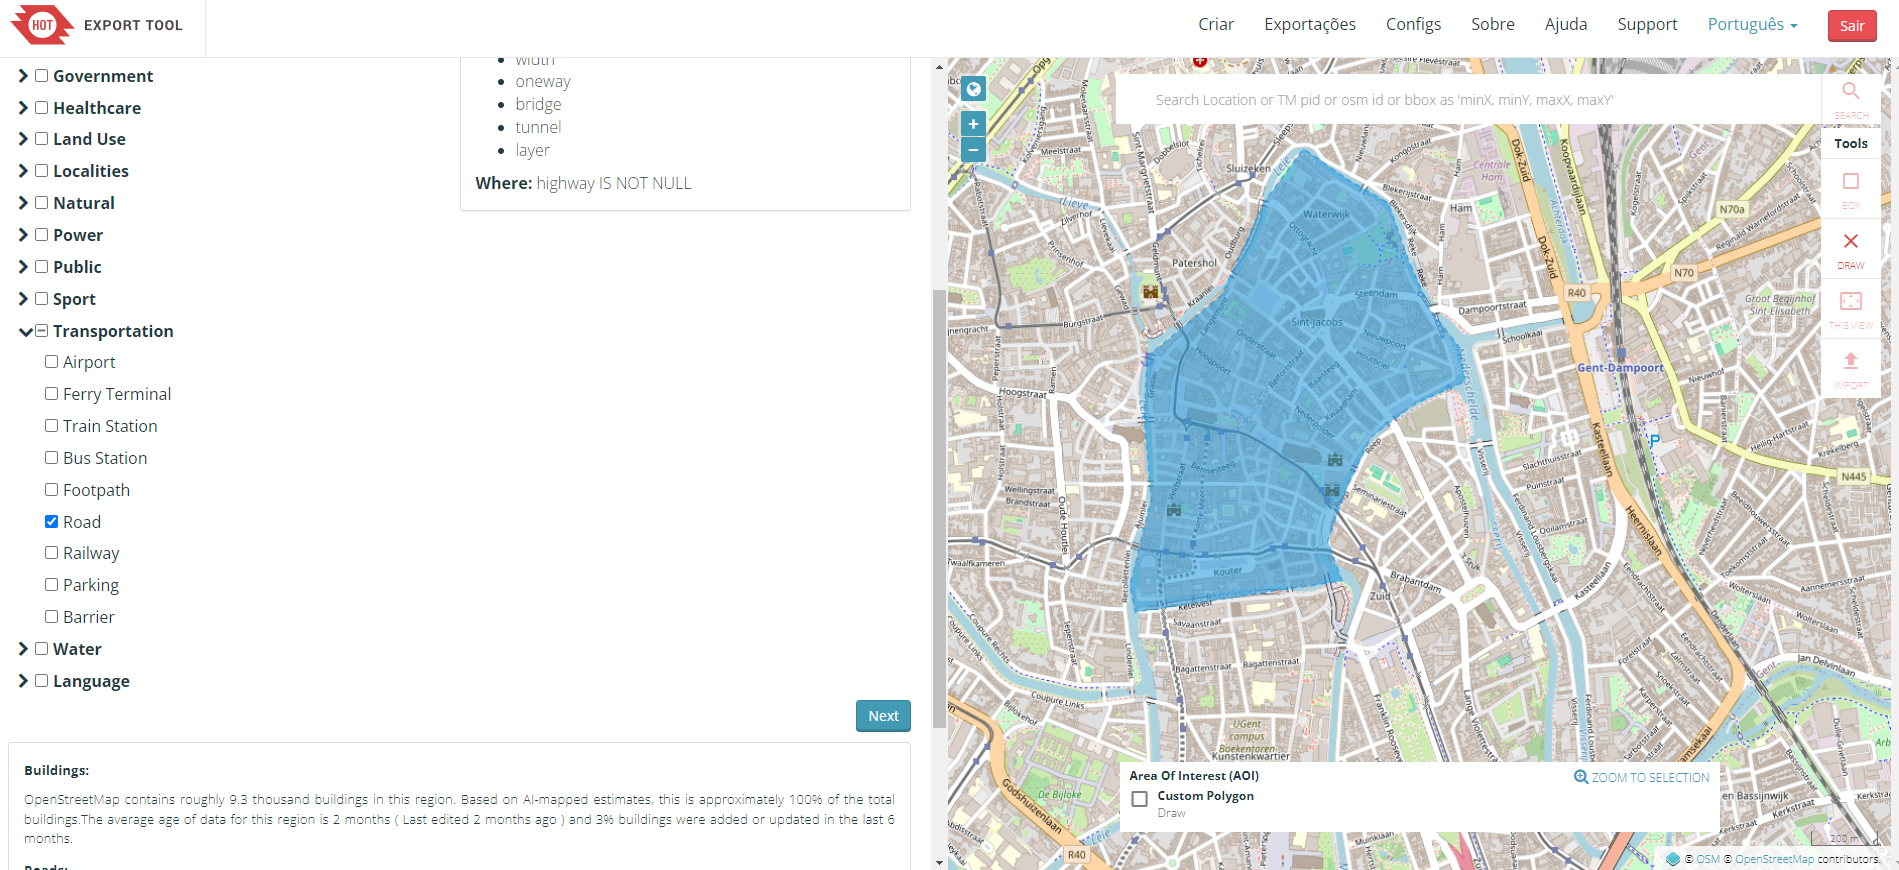
\includegraphics{images/clipboard-1441436716.png}

After the export, you can read in R using the \texttt{sf} package:

\begin{Shaded}
\begin{Highlighting}[]
\NormalTok{Gent }\OtherTok{=}\NormalTok{ sf}\SpecialCharTok{::}\FunctionTok{st\_read}\NormalTok{(}\StringTok{"data/Gent\_center.gpkg"}\NormalTok{, }\AttributeTok{quiet =} \ConstantTok{TRUE}\NormalTok{)}

\NormalTok{mapview}\SpecialCharTok{::}\FunctionTok{mapview}\NormalTok{(Gent, }\AttributeTok{zcol =} \StringTok{"highway"}\NormalTok{)}
\end{Highlighting}
\end{Shaded}

\includegraphics{open-data_files/figure-pdf/unnamed-chunk-1-1.png}

\subsection{OSM in R}\label{osm-in-r}

There are also some R packages that can help you to download and work
with OpenStreetMap data, such as:

\begin{itemize}
\tightlist
\item
  \href{https://cran.r-project.org/web/packages/osmdata/index.html}{\texttt{osmdata}}
\item
  \href{https://docs.ropensci.org/osmextract}{\texttt{osmextract}}
\end{itemize}

This is an example of how to download OpenStreetMap road network data
using the \texttt{osmextract} package:

\begin{Shaded}
\begin{Highlighting}[]
\FunctionTok{library}\NormalTok{(osmextract)}
\NormalTok{OSM\_Malta }\OtherTok{=} \FunctionTok{oe\_get\_network}\NormalTok{(}\AttributeTok{place =} \StringTok{"Malta"}\NormalTok{) }\CommentTok{\# it will geocode the place}

\NormalTok{Malta\_main\_roads }\OtherTok{=}\NormalTok{ OSM\_Malta }\SpecialCharTok{|\textgreater{}} 
  \FunctionTok{filter}\NormalTok{(highway }\SpecialCharTok{\%in\%} \FunctionTok{c}\NormalTok{(}\StringTok{"primary"}\NormalTok{, }\StringTok{"secondary"}\NormalTok{, }\StringTok{"tertiary"}\NormalTok{, }\StringTok{"trunk"}\NormalTok{))}

\FunctionTok{plot}\NormalTok{(Malta\_main\_roads[}\StringTok{"highway"}\NormalTok{])}
\end{Highlighting}
\end{Shaded}

\begin{center}
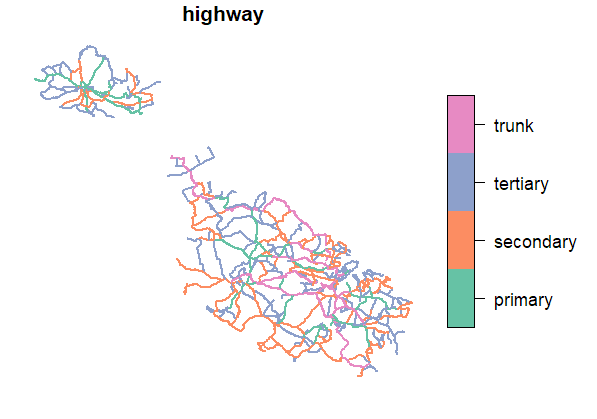
\includegraphics{images/malta_roads.png}
\end{center}

\section{Transportation Services'
Data}\label{transportation-services-data}

\subsection{GTFS}\label{gtfs}

\subsection{National Access Points}\label{national-access-points}

The European Union has a directive that requires the member states to
provide access to transportation data. Data includes not only
\textbf{Public Transportation} data, but also \textbf{road network}s,
car \textbf{parking}, and other transportation-related information.

\href{https://transport.ec.europa.eu/transport-themes/smart-mobility/road/its-directive-and-action-plan/national-access-points_en}{List
of the European Union members states with National Access Points for
Transportation data}

Example of Bus services data in Belgium:

\begin{figure}[H]

{\centering 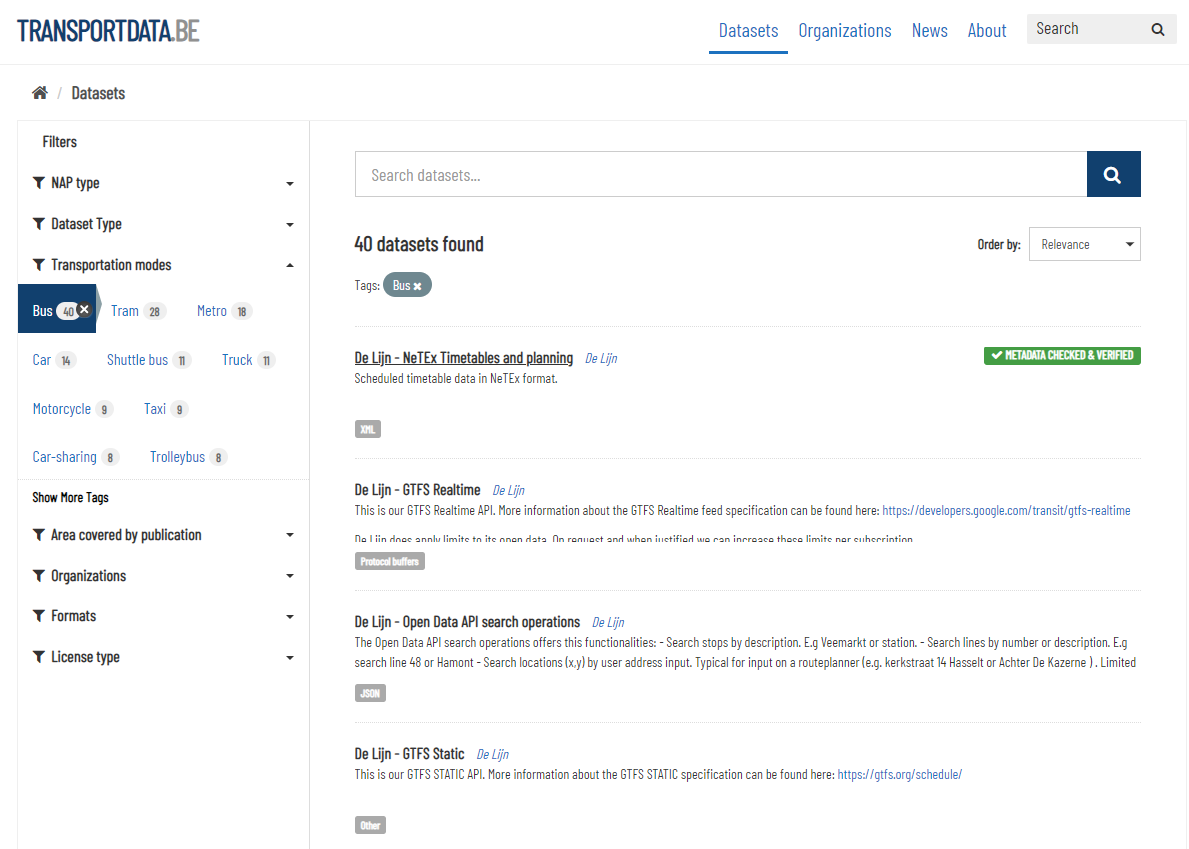
\includegraphics{images/clipboard-3645209787.png}

}

\caption{Source: Transport Data Belgium}

\end{figure}%

\chapter{Urban Accessibility with R}\label{urban-accessibility-with-r}

The module ``\textbf{A crash course on urban accessibility with R}'',
lectured by
\href{https://ipeagit.github.io/access_workshop_eit_2024/\#about-the-instructor}{Rafael
H. M. Pereira}, has it's own website with materials.

\begin{tcolorbox}[enhanced jigsaw, breakable, left=2mm, colframe=quarto-callout-note-color-frame, leftrule=.75mm, bottomrule=.15mm, arc=.35mm, rightrule=.15mm, colback=white, opacityback=0, toprule=.15mm]
\begin{minipage}[t]{5.5mm}
\textcolor{quarto-callout-note-color}{\faInfo}
\end{minipage}%
\begin{minipage}[t]{\textwidth - 5.5mm}

Please access it here:
\url{https://ipeagit.github.io/access_workshop_eit_2024/}

\end{minipage}%
\end{tcolorbox}

\begin{figure}[H]

{\centering 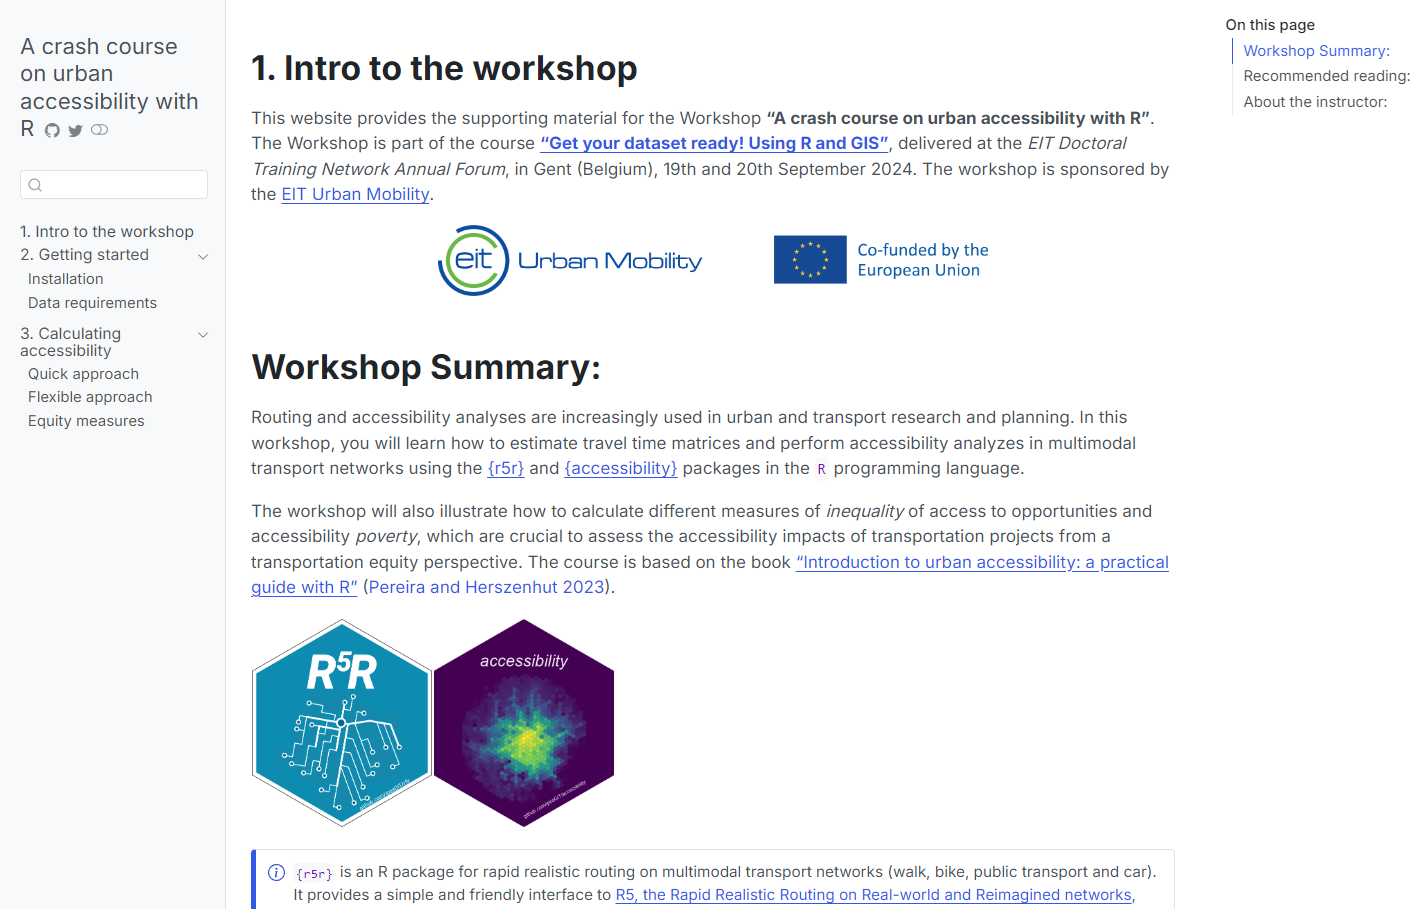
\includegraphics{images/clipboard-4241488434.png}

}

\caption{Screenshot of the website for this learning module.}

\end{figure}%

\section*{About the instructor}\label{about-the-instructor}
\addcontentsline{toc}{section}{About the instructor}

\markright{About the instructor}

\textbf{Rafael H. M. Pereira}\\
\emph{Head of Data Science}\\
Institute for Applied Economic Research (Ipea), Brazil\\
\href{https://www.urbandemographics.org/about/}{Website} \textbar{}
\href{https://scholar.google.com.br/citations?user=dbRivsEAAAAJ&hl}{Google
Scholar} \textbar{} \href{https://x.com/UrbanDemog}{Twitter} \textbar{}
\href{https://www.linkedin.com/in/rafael-h-m-pereira/}{Linkedin}
\textbar{}

\textbf{Short bio}

Rafael H. M. Pereira is a senior researcher in the fields of urban
analytics, spatial data science and transport studies at the Institute
for Applied Economic Research (Ipea), Brazil. His research looks broadly
at how urban policies and technologies shape the spatial organization of
cities, human mobility as well as their impacts on social and health
inequalities. Some of his key contributions to the fields of urban
analytics and planning involve the development of new methods and
open-source computational tools to the study of urban systems and
transportation networks. These contributions emerge from substantive
interests around social justice and sustainability issues in urban
development, with particular focus on transportation equity and
inequalities in access to opportunities, and the environmental impacts
of built environments and mobility patterns. With a background in
Sociology and Demography, Dr.~Pereira obtained his PhD in Geography from
the Transport Studies Unit at Oxford University.

\bookmarksetup{startatroot}

\chapter*{References}\label{references}
\addcontentsline{toc}{chapter}{References}

\markboth{References}{References}

\phantomsection\label{refs}
\begin{CSLReferences}{1}{0}
\bibitem[\citeproctext]{ref-IMOB}
INE. 2018. {``Mobilidade e Funcionalidade Do Território Nas {Áreas
Metropolitanas do Porto e de Lisboa}: 2017.''} Lisboa: {Instituto
National de Estatística}.
\url{https://www.ine.pt/xportal/xmain?xpid=INE&xpgid=ine_publicacoes&PUBLICACOESpub_boui=349495406&PUBLICACOESmodo=2&xlang=pt}.

\bibitem[\citeproctext]{ref-INEcensus}
---------. 2022. {``{Censos 2021- XVI Recenseamento Geral da População.
VI Recenseamento Geral da Habitação}.''} Lisboa: {Instituto National de
Estatística}. \url{https://censos.ine.pt/xurl/pub/65586079}.

\bibitem[\citeproctext]{ref-stplanr}
Lovelace, Robin, and Richard Ellison. 2018. {``Stplanr: A Package for
Transport Planning.''} \emph{{The R Journal}} 10 (2): 10.
\url{https://doi.org/10.32614/RJ-2018-053}.

\bibitem[\citeproctext]{ref-od}
Lovelace, Robin, and Malcolm Morgan. 2024. \emph{Od: Manipulate and Map
Origin-Destination Data}. \url{https://github.com/itsleeds/od}.

\bibitem[\citeproctext]{ref-sf}
Pebesma, Edzer, and Roger Bivand. 2023. \emph{Spatial Data Science: With
Applications in {R}}. Boca Raton: Chapman; Hall/CRC.
\url{https://doi.org/10.1201/9780429459016}.

\bibitem[\citeproctext]{ref-centr}
Zomorrodi, Ryan. 2024. \emph{Centr: Weighted and Unweighted Spatial
Centers}. \url{https://ryanzomorrodi.github.io/centr/}.

\end{CSLReferences}




\end{document}
